% \documentclass[journal]{vgtc}                % final (journal style)
\documentclass[review,journal]{vgtc}         % review (journal style)
% \documentclass[widereview]{vgtc}             % wide-spaced review
%\documentclass[preprint,journal]{vgtc}       % preprint (journal style)


\ifpdf%                                % if we use pdflatex
  \pdfoutput=1\relax                   % create PDFs from pdfLaTeX
  \pdfcompresslevel=9                  % PDF Compression
  \pdfoptionpdfminorversion=7          % create PDF 1.7
  \ExecuteOptions{pdftex}
  \usepackage{graphicx}                % allow us to embed graphics files
  \DeclareGraphicsExtensions{.pdf,.png,.jpg,.jpeg} % for pdflatex we expect .pdf, .png, or .jpg files
\else%                                 % else we use pure latex
  \ExecuteOptions{dvips}
  \usepackage{graphicx}                % allow us to embed graphics files
  \DeclareGraphicsExtensions{.eps}     % for pure latex we expect eps files
\fi%

\graphicspath{{figures/}{pictures/}{images/}{./}} % where to search for the images

\usepackage{microtype}                 % use micro-typography (slightly more compact, better to read)
\PassOptionsToPackage{warn}{textcomp}  % to address font issues with \textrightarrow
\usepackage{textcomp}                  % use better special symbols
\usepackage{mathptmx,amsmath,amssymb,amsthm}             % use matching math font
\usepackage{times}                     % we use Times as the main font
\renewcommand*\ttdefault{txtt}         % a nicer typewriter font
\usepackage{cite}                      % needed to automatically sort the references
\usepackage{tabu}                      % only used for the table example
\usepackage{booktabs}                  % only used for the table example
\usepackage{color}
\usepackage{algorithm, algorithmicx}
\usepackage[noend]{algpseudocode}
\usepackage{color}
\usepackage{enumitem}
\usepackage{float}
\usepackage{balance}% for  \balance command ON LAST PAGE  (only there!)


\newtheorem{problem}{Problem}
\newtheorem{lemma}{Lemma}
\newtheorem{theorem}{Theorem}
\newcommand{\Bo}[1]{{\color{red} Bo: #1}}

\newcommand{\D}{\mathsf{T}}
\newcommand{\V}{\mathsf{V}}
\newcommand{\oR}{\mathsf{R}}
\newcommand{\U}{\mathsf{U}}
\newcommand{\vats}{\mathsf{VFGS}}
\newcommand{\rand}{\mathsf{RAND}}
\newcommand{\full}{\mathsf{FULL}}
\newcommand{\avats}{\mathsf{VFGS}^{+}}
\newcommand{\cavats}{\mathsf{VFGS}^{+}\mathsf{CE}}
\newcommand{\sz}{\textsf{Shenzhen}}
\newcommand{\pt}{\textsf{Porto}}

\newcommand{\stitle}[1]{\vspace*{0.4em}\noindent{\bf #1:\/}}
\newcommand{\sstitle}[1]{\vspace*{0.4em}\noindent{\bf #1\/.}}


\newcommand{\squishlist}{
 \begin{list}{$\bullet$}
 { \setlength{\itemsep}{0pt}
   \setlength{\parsep}{3pt}
   \setlength{\topsep}{3pt}
   \setlength{\partopsep}{0pt}
   \setlength{\leftmargin}{1.2em}
   \setlength{\labelwidth}{1em}
   \setlength{\labelsep}{0.6em}
 }
}
\newcommand{\squishend}{
 \end{list}
}



\onlineid{1029}

%% declare the category of your paper, only shown in review mode
\vgtccategory{Research}
%% please declare the paper type of your paper to help reviewers, only shown in review mode
%% choices:
%% * algorithm/technique
%% * application/design study
%% * evaluation
%% * system
%% * theory/model
\vgtcpapertype{algorithm/technique}

%% Paper title.
%\title{Visualization aware trajectory sampling for urban traffic data}
%\title{Visualization-aware Sampling for Big Trajectory Data}
% \title{Visual Quality Guaranteed Sampling for \\ Large Trajectory Data Visualization}
\title{Visual Fidelity Guaranteed Sampling for \\ Large Trajectory Data Visualization}


%%% indicate IEEE Member or Student Member in form indicated below
%\author{Roy G. Biv, Ed Grimley, \textit{Member, IEEE}, and Martha Stewart}
%\authorfooter{
%%% insert punctuation at end of each item
%\item
% Roy G. Biv is with Starbucks Research. E-mail: roy.g.biv@aol.com.
%\item
% Ed Grimley is with Grimley Widgets, Inc.. E-mail: ed.grimley@aol.com.
%\item
% Martha Stewart is with Martha Stewart Enterprises at Microsoft
% Research. E-mail: martha.stewart@marthastewart.com.
%}
%
%%other entries to be set up for journal
%\shortauthortitle{Biv \MakeLowercase{\textit{et al.}}: Global Illumination for Fun and Profit}
%%\shortauthortitle{Firstauthor \MakeLowercase{\textit{et al.}}: Paper Title}

%% Abstract section.
\abstract{
%\QM{Line-based visualization has been widely used to present trajectory data. However, when the data size grows very large, it will take a considerable amount of time to render the graphics. Sampling techniques can mitigate the problem by directly shrinking the dataset, thus to reduce the rendering work of graphic devices. However, the traditional sampling techniques may lead to the loss of visual information and cannot directly be applied in line-based trajectory visualization. This work presents a novel approach, visual quality guaranteed sampling(VQGTS), specifically for the data reduction of large trajectory data visualization. We first propose a loss function to measure the visual quality loss between the visualization of the sub-dataset and the whole dataset. Then we minimize the loss function by transforming it as an optimization problem and propose efficient solutions. Several parameters and color encoding which can empower the effectiveness are discussed. The experiments on several large trajectory datasets demonstrate the effectiveness of the proposed method.  The user study further shows the usability of our methods in the exploration of large trajectory data.}
%\ZW{
%In this work, we present a novel sampling approach for line-based visualization of large trajectory data, targeting at maximizing the visual fidelity of sampled trajectory visualization.
%We introduce a new measurement of fidelity loss using pixel-oriented proximity between two visualization images.
%From the metric we formulate the sampling as an NP-hard optimization problem, and develop an efficient algorithm $-$ VFMS??, to approximate the optimal solution.
%VFMS encapsulates various control parameters including sampling rate and level of details (LODs), which complement with color coding to empower the effectiveness of trajectory visualization.
%We conduct a formal study to compare VFMS with state-of-the-art sampling methods on several large trajectory datasets.
%The experiments show that our approach improves visual fidelity by xxx\% (numbers?) meanwhile keeps computational efficiency.
%Qualitative user studies further demonstrate the feasibility of our approach in XXX (concrete applications?).}
% Visualizing large-scale trajectories is the core subroutine in many smart city applications, e.g., traffic management, route recommendation.
% However, it is very challenging as (i) the large trajectory data size, (ii) the limited rendering capability of graphics device, and (iii) visual clutter in data visualization.
% In this work, we propose a visual fidelity guaranteed sampling approach for large-scale line-based trajectory visualization.
% Specifically, we first define a novel fidelity loss function to capture the visual difference between two visualization results.
% We then prove that it is NP-hardness to select a sized-$k$ subset of trajectories with minimal visual fidelity loss.
% Next, we devise an approximate algorithm $\vats$ with a suite of optimization techniques, which returns visual fidelity quality guaranteed visualization result efficiently.
% Moreover, we further improve the visual effectiveness of $\vats$ by reduce visual clutter in large data visualization.%taking human perception ability and visual clutter issue into consideration.
% We conduct extensive experimental studies to demonstrate the effectiveness of our proposal on real-world trajectory datasets.
% In addition, qualitative user studies further illustrate the superiority of our approach in various applications, e.g., region center identification, reachable route inspection, traffic flow comparison.
\ZW{
Visualizing large trajectory data surfers from limited rendering capability and visual clutter issues.
Sampling can effectively mitigate the issues, yet existing methods generally adopt random sampling strategy that has an attenuating effect on visual fidelity.
In this work, we propose a \QM{\textit{\textbf{visual fidelity guaranteed sampling}}} ($\avats$) algorithm for line-based visualization of large trajectory data.
We first define a novel fidelity loss function to capture the visual difference between two visualizations.
We prove that it is NP-hard to select a sized-$k$ subset of trajectories with minimal visual fidelity loss.
Next, we devise an approximation algorithm $\vats$ with a suite of optimization techniques, which returns fidelity-guaranteed visualizations efficiently.
Moreover, we improve the effectiveness of $\vats$ by taking human perception and cluttering degree into consideration.
We conduct extensive experimental studies to demonstrate the effectiveness of our method on real-world trajectory datasets.
Qualitative user studies further illustrate the superiority of $\vats$ in various applications, e.g., traffic flow detection, and reachable route discovery.
}
}


\keywords{Trajectory visualization, quality guaranteed sampling, visual fidelity}


\teaser{
  \centering
  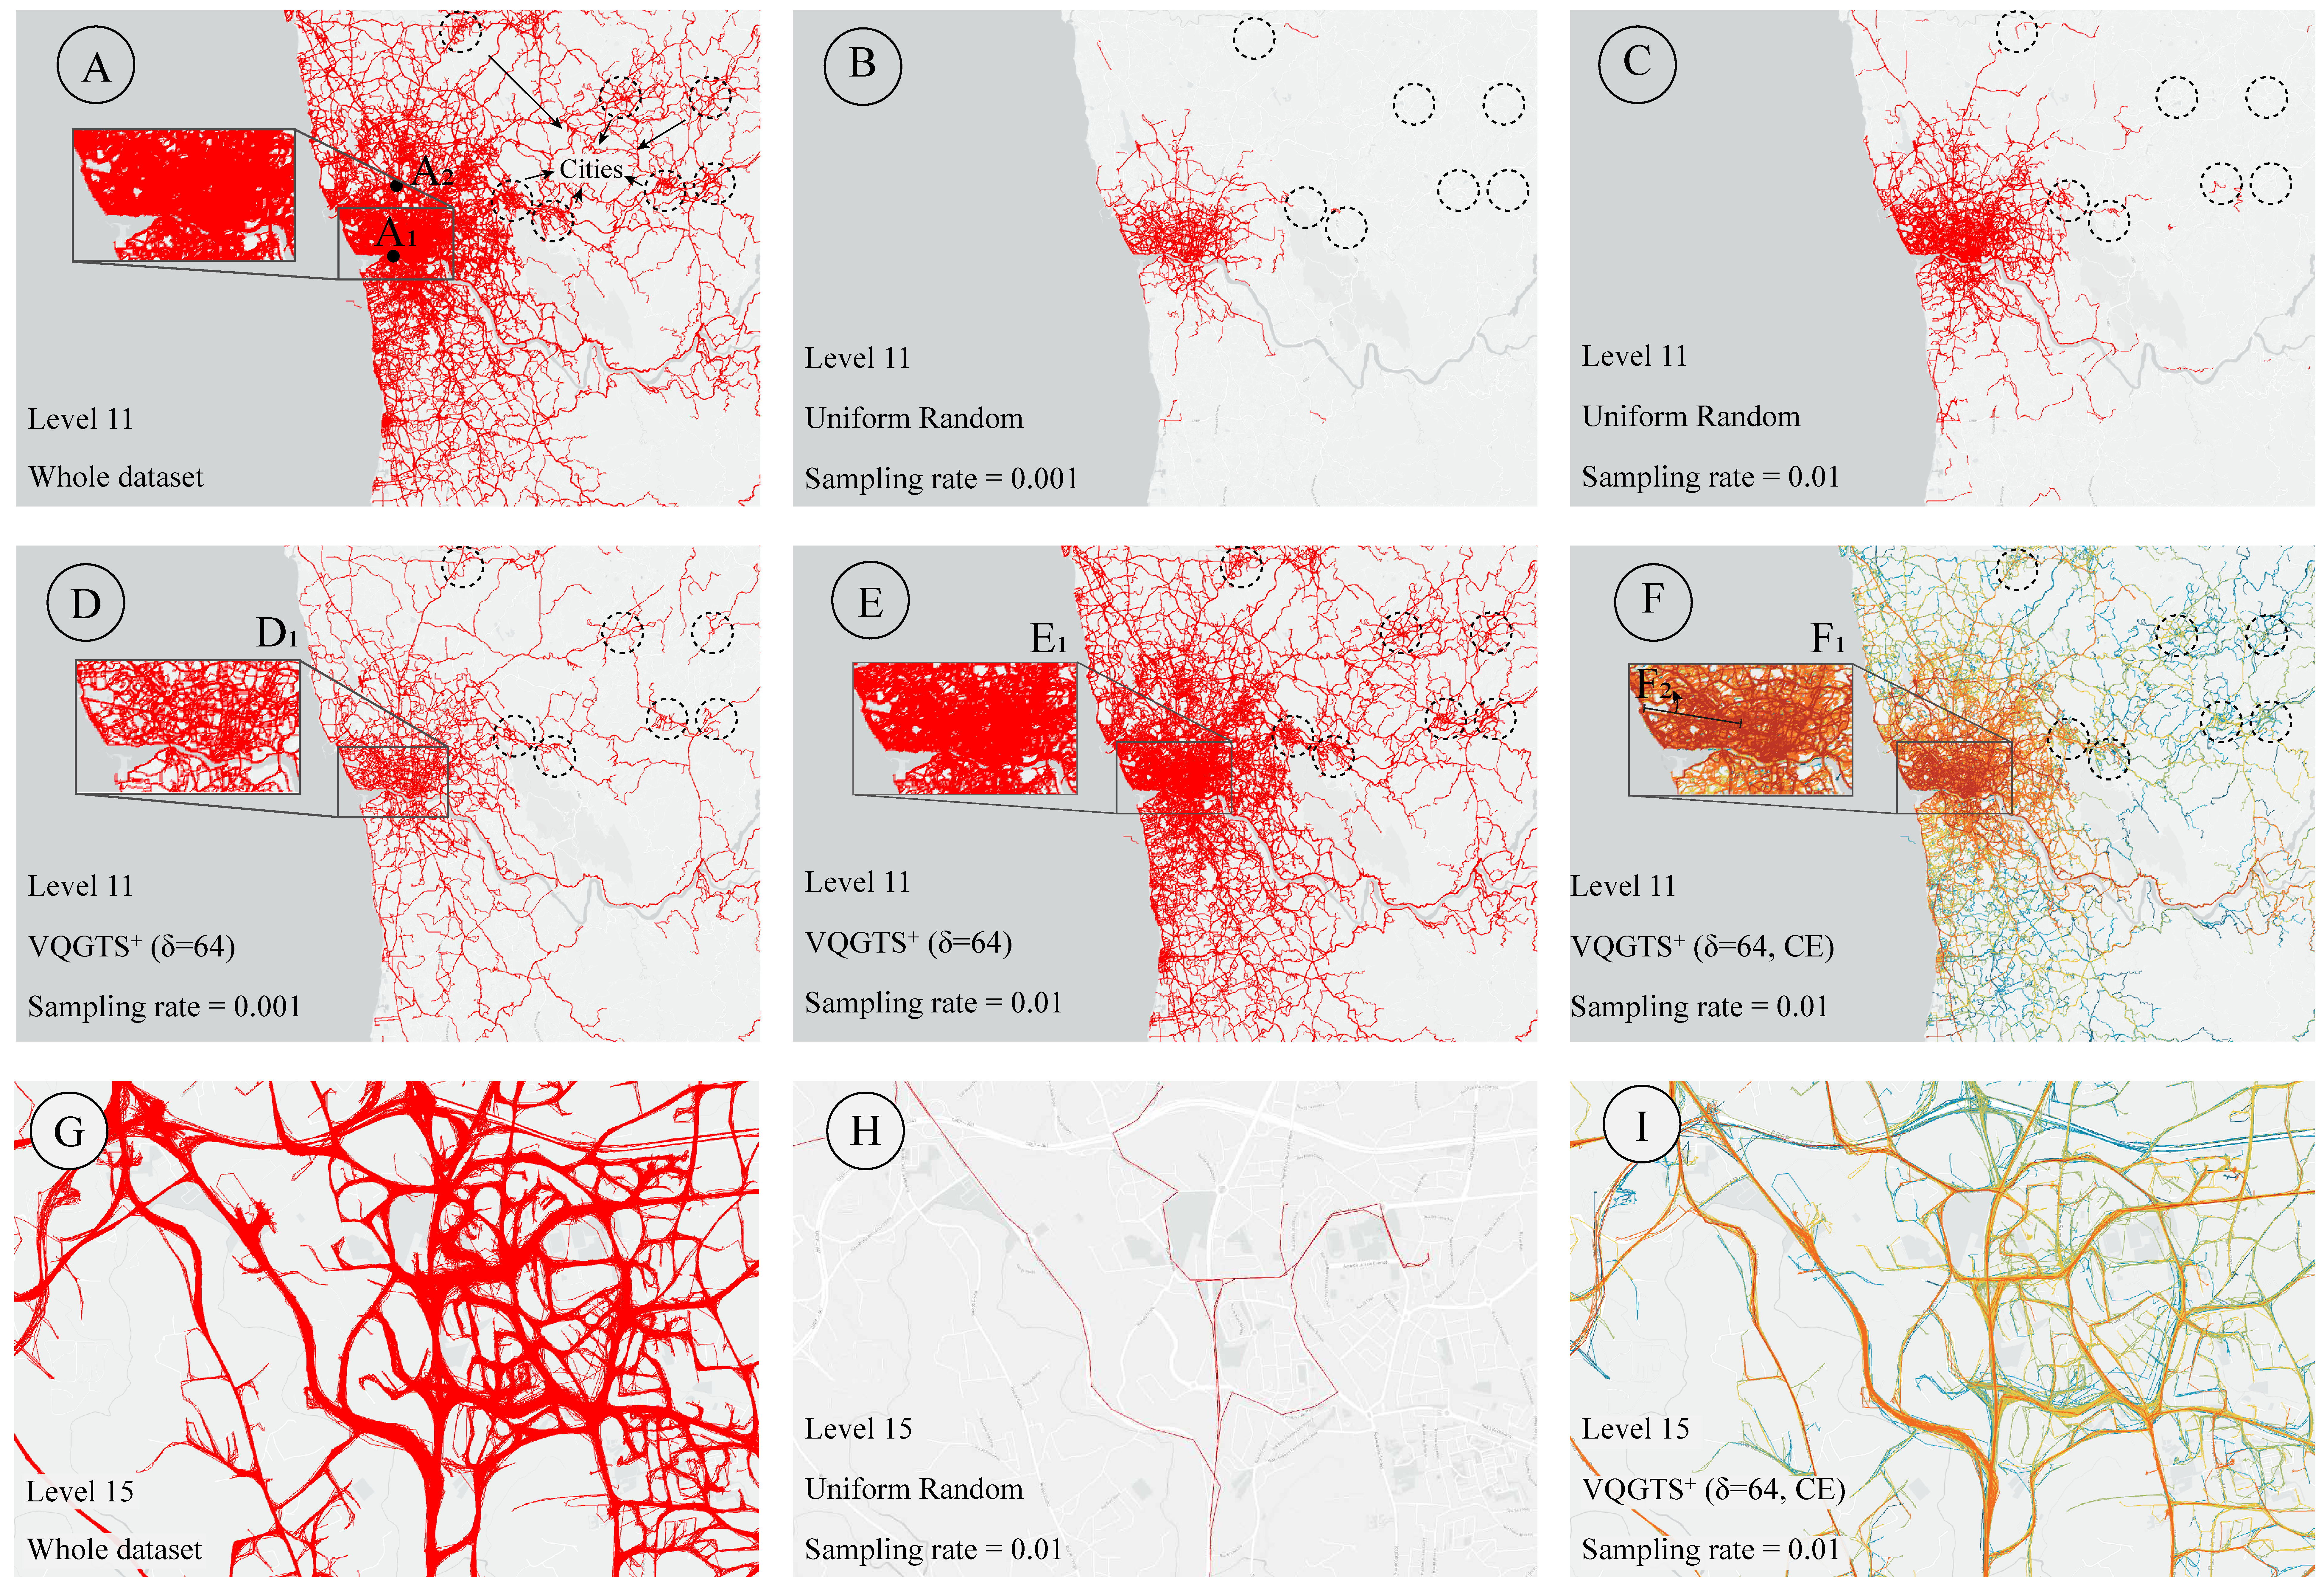
\includegraphics[width=0.9\linewidth]{Teaser.pdf}
  \vspace{-3mm}
  \caption{
  % Visualization results. (I) at zoom level 11, (A) is the visualization result of the \pt{} taxi trajectory dataset.
  %  B and C are visualization results of uniform random sampling with sampling rate $0.1\%$ and $1\%$, respectively.
  %  D, E, F are the visualizations of our advanced approach $\avats$ with different parameters.
  %  (II) G, H, and I are the visualizations of full \pt{} dataset, uniform random sampling $\rand$ result set, and our proposal $\avats$ result set at zoom level 15, respectively.
\ZW{
Comparison of random sampling and $\avats$. (i) A is the visualization of the \pt{} taxi trajectory dataset at zoom level 11.
B and C are visualizations of random sampling with sampling rate $0.1\%$ and $1\%$, respectively.
D, E, F are visualizations of our proposed $\avats$ with different parameters.
(ii) G, H, and I are visualizations of the whole \pt{} dataset, random sampling with sampling rate $1\%$, and $\avats$ with sampling rate $1\%$ at zoom level 15, respectively.
}
   }
	\label{fig:teaser}
}



\vgtcinsertpkg


\definecolor{orange}{RGB}{242, 101, 34}
\definecolor{purple}{RGB}{197,27,125}
%---------------------------------------------------

\newcommand{\QM}[1]{{\color{red}{#1}}}

\newcommand{\ZW}[1]{{\color{blue}{#1}}}

\newcommand{\UC}[1]{{\color{red}{#1}}}

\newcommand{\NH}[1]{{\color{purple}{#1}}}

\newcommand{\TB}[1]{{\color{purple}{#1}}}

\begin{document}


%\firstsection{Introduction}

\maketitle

%\vspace{-2mm}
\section{Introduction}\label{sec:intro}
Nowadays, the widely used location-acquisition devices lead to an explosive increase of the movement data (i.e., GPS trajectories) from urban moving objects, e.g., cars, sharing bikes, and pedestrians.
Trajectory visual analysis have been employed in many smart city applications, e.g.,  traffic management~\cite{wang2014visual}, urban planning~\cite{tang2017efficient}, route recommendation~\cite{zheng2011learning} and location-based services~\cite{liu2016smartadp, zheng2010collaborative}.
Line-based trajectory visualization, i.e., connecting the GPS points of a movement object by polylines, is a popular and conventional visualization method~\cite{chen2015survey}.
%we should focus on line-based trajectory visualization here.
However, efficient and effective large-scale line-based trajectory visualization is challenging.
The reasons are (i) large trajectory data size, (ii) limited rendering ability of graphics device and (iii) visual clutter in large data visualization.
We elaborate them as follows:

\stitle{Large trajectory data size} The trajectory data size is extremely huge.
For example, Shenzhen has 24,237 taxis and generates more than 82.8 millions GPS locations (e.g., taxi trajectories) in each day~\cite{sz}. %\footnote{\url{http://jtys.sz.gov.cn/}}.
In New York City, it has 13,000 taxis, averagely, they carry over 1.0 million passengers and make 500,000 trips per day~\cite{ferreira2013visual}.

\stitle{Limited rendering ability of graphics device}
Rendering refers to the use of hardware device (e.g., GPU) in the automatic generation of visualization result.
However, due to the hardware limitation, the rendering ability of modern commodity GPU is limited.
We did a benchmark experiment to evaluate the rendering ability of NVIDIA GeForce GTX 1080 with 8GB video memory.
We vary the number of trajectories from 1,000 to 1 millions, which are randomly selected from \pt{} taxi trajectory dataset~\cite{pt}.%\footnote{\url{http://www.geolink.pt/ecmlpkdd2015-challenge/dataset.html}}.
The experimental results are summarized in Table~\ref{tab:gpu}.
Obviously, it cannot support interactive visual exploration in large-scale trajectory dataset, e.g.,
it needs 13.95 seconds to render 1 million trajectories with 32.67 millions GPS points (almost 40\% of \sz{} taxi trajectory GPS points in one day).
Moreover, the rendering cost is linear with the input data trajectories.
Thus, it is impractical to visualize billion-level GPS points via the commodity GPUs.

\begin{table}
	\centering
    \small
	\caption{Visualization rendering cost of GTX 1080}
	\begin{tabular}{|c|c|c|} \hline
		No. of trajectories & No. of GPS points & Rendering time (s) \\ \hline
		1,000& 32,648 & 0.016\\ \hline
		10,000& 331,583 & 0.143\\ \hline
		100,000& 3,262,278 & 1.416\\ \hline
		1,000,000& 32,660,845 & 13.950\\ \hline
	\end{tabular}	\label{tab:gpu}
\end{table}

\stitle{Visual clutter in data visualization}
Visual clutter is a common issue in data visualization~\cite{clutter}.
Fig.~\ref{fig:teaser}A is the visualization result of the full \pt{} taxi trajectory dataset.
Intuitively, the region shown in the embedded figure of A suffers visual clutter issue seriously,
i.e., the road network almost cannot be recognized in it,
which hinders the abilities of human-users to explore the dataset and identify the underlying data insights.



To overcome the above challenges, several visualization approaches have been proposed in the literature.
Unfortunately, none of them could address these three challenges simultaneously and perfectly.
In particular, the spatial aggregation based approaches~\cite{zeng2013visualizing,von2015mobilitygraphs} preprocess the massive movement data, and visualize the results after preprocessing.
The aggregation based methods ignored the visual clutter in raw spatial data as they only visualize the aggregated/preprocessed results.
In other words, their visualization results may lose detial information in raw data.
%These approaches alleviate the large data size and limited rendering ability issues in large-scale spatial data visualization.
%Nevertheless, they ignored the visual clutter issue in raw spatial data as they only visualize the aggregated/preprocessed results.
In recent years, many visualization research works are proposed to address visual clutter,
e.g., edge bundling~\cite{zeng2019route, thony2015vector} and density map~\cite{lampe2011interactive, scheepens2011interactive}.
However, these works neither focus on line-based trajectory visualization nor designed for large-scale trajectory dataset.

Sampling techniques is a de-facto standard for large-scale data analysis in both database and visualization community.
In general, it samples a subset of data from the raw large-scale dataset, then it could be rendered efficiently by the graphics device.
For example, ScalaR~\cite{battle2013dynamic} employs a reduction layer between visualization layer and data management layer.
The reduction layer embedded an uniform random sampling algorithm to sample data randomly when the query results are large enough.
It then reduces the amount of data to be visualized.
However, the uniform random sampling method does not work well in our large trajectory data visualization problem as it does not have any guarantees about the sampling results.
Take Fig.~\ref{fig:teaser}(B) and (C) as an example,
they are the visualization results of uniform random sampling method on \pt{} taxi trajectory dataset with sampling rate $0.1\%$ and $1\%$, respectively.
Visually, both visualized results cannot capture the overview of the input data, as shown in Fig.~\ref{fig:teaser}(A).

In database community,  Park et al. devised a visualization-aware sampling algorithm (VAS) for large-scale scatter points visualization problem in~\cite{park2016visualization},
which offers theoretical quality guarantee on the visualization result.
However, the VAS techniques cannot be adapted to our problem as  (i) trajectory data is  more complex than scatter points (e.g., varying lengths, lack of compact representation),
and  (ii) the formulated visualization quality measure function in~\cite{park2016visualization} is only for scatter points, it cannot be used to measure the quality of trajectory visualization results.

In this work, we propose visual fidelity guaranteed sampling approaches for the line-based trajectory visualization problem,
which kills three birds (i.e., the above three challenges) by one stone.
The technical challenges of our proposals are
(i) how to define visual fidelity guarantee theoretically?
(ii) how to devise an efficient sampling algorithm which offers visual fidelity guarantee on the visualization result,
and (iii) how to overcome the visual clutter in large trajectory visualization.
Specifically, we first define a novel the visual fidelity loss function between two visualization results formally.
With the visual fidelity loss function, we then prove it is NP-hardness to select a sized-$k$ subset of trajectories which has the minimal visual fidelity loss.
Next, we devise an approximate algorithm ($\vats$) which returns a sized-$k$ subset of trajectories and offers theoretical visual fidelity guarantee on the returning result.
Last, we address the visual clutter issue explicitly and overcome it by taking data distribution and human perception capability into consideration in the advance approach ($\avats$).
Fig.~\ref{fig:teaser}(D) and (E) show the visualization results of our proposal $\avats{}$ on \pt{} taxi trajectory dataset with sampling rate $0.1\%$ and $1\%$, respectively.
Obviously, the visualization fidelity of them (comparing with the visualization result of full dataset in Fig.~\ref{fig:teaser}(A)) is much better than
the uniform random sampling visualization results with the same sampling rate, see (B) and (C) in Fig.~\ref{fig:teaser}.
Fig.~\ref{fig:teaser}(F) is the returning result of our proposal which colors the trajectories with different representativeness.
It has the same input parameters of Fig.~\ref{fig:teaser}(E).
Intuitively, the visual clutter in Fig.~\ref{fig:teaser}(A) and (E) is almost removed in Fig.~\ref{fig:teaser}(F).
In addition, our proposals are robustness with different zoom levels.
Fig.~\ref{fig:teaser}(G), (H), and (I) depict the visualization results of the full \pt{} dataset, the returning result of uniform random sampling $\rand$ and the returning result of $\avats$ with color encoding at zoom-level 15, e.g., we can obtain them by zooming in the visualization result in Fig.~\ref{fig:teaser}(A), (C), and (F), respectively.
Intuitively, the visualization result of our proposal $\avats$ in Fig.~\ref{fig:teaser}(F) outperforms the uniform random sampling method $\rand$ in Fig.~\ref{fig:teaser}(H) significantly.
It even performs better than Fig.~\ref{fig:teaser}(G), the visualized result of the full dataset, as it reduces visual clutter in G by using color encoding scheme to capture the representativeness of different roads.

The contributions of this paper are:
\setlist{nolistsep}
\begin{itemize}[noitemsep]
  \item We formulate the visual fidelity guaranteed sampling problem for large trajectory data visualization, and prove it is NP hard in Section~\ref{sec:pro}.
  \item We devise an approximation algorithm for it with a suite of optimization techniques, e.g., submodularity, lazy computing in Section~\ref{sec:sol}.
  \item We propose an advanced approach to further enhance the effectiveness of our approximate algorithm, which address the visual clutter by introducing perception tolerance parameter,
  and encodes the representativeness of each road by different colors in Section~\ref{sec:aa}.
  \item We conduct extensive experiments on real-world trajectory datasets to demonstrate the superiority of our proposals in Section~\ref{sec:exp}. Especially, we conduct qualitative user studies to show their effectiveness on three real-world applications.
\end{itemize}

%Our proposal demonstrates their superiority over existing methods
%With the same sampling set size($1\%$), the proposed method generates a higher-fidelity visualization and .

%With the loss function, we analyze the hardness of the problem, and devise a visual quality guaranteed sampling algorithm for it.
%Figure~\ref{fig:compare} depicts an comparison among the ground truth,  uniform random sampling and our proposed method.
%With the same sampling set size($1\%$), the proposed method generates a higher-fidelity visualization and support the multi-resolution very well.
%At last, color encoding are applied to enhance the distribution of trajectories.

%


%\TB{Visualizing a large collection of trajectories are used frequently in map service or smart city applications.}
%The most popular and conventional method is the line-based visualization~\cite{chen2015survey}: connecting the passing points of movement objects by polylines.
%To handle the big dataset, many visualization products such as Spotfire~\footnote{\url{https://www.tibco.com/products/tibco-spotfire}}
%and Tableau~\footnote{\url{https://www.tableau.com/}} support advanced database management systems as a ``backend'' for the efficient data processing the query.
%The current visualization tools always don't scale well for the presentation of very large trajectory dataset due to the two challenges,
%visual clutter and limited rendering speed, which hinders the abilities of human-users for interactively exploring the dataset and identifying the movement patterns.
%In recent years, most of the visualization research works mainly try to address the visual clutter issue by proposing new techniques such as the
%spatial aggregation~\cite{zeng2013visualizing, von2015mobilitygraphs}, edge bundling~\cite{zeng2019route, thony2015vector} and density map~\cite{lampe2011interactive, scheepens2011interactive}.
%Instead, in this paper, we focus on the challenge of inefficient rendering in the large trajectory dataset by involving data sampling techniques.

%It is time consuming to generate very simple visualization when the data size become very large. Using Porto taxi data ~\footnote{\url{http://www.geolink.pt/ecmlpkdd2015-challenge/dataset.html}} as an example, Table~\ref{table:rendering_time} demonstrates the rendering time at each dataset size. \ZW{shall also mention which rendering toolkit is used here.} It shows that normal method takes more than 14 minutes (\ZW{seconds?}) to generate the graphics for 1 million trajectories, which is far beyond the human-acceptable response time for the interactive exploration~\cite{shneiderman1984response}.
%One work closely related to ours is ScalaR~\cite{battle2013dynamic}, which adds a reduction layer between visualization layer and data management layer. The reduction layer uses an uniform random sampling method to sample data once the query results are large enough, thus to reduce the amount of data to be visualized.
%Further more, Park et al. propose VAS~\cite{park2016visualization} which implements new sampling techniques to guarantee the visual quality.
%However, these sampling techniques are designed for the simple dataset, and have been approved effective in scatter plot or map plot.
%However, the trajectory sampling is more challenge due to the complexity of data form(e.g. varying lengths, lack of compact representation, difficulty in measuring the similarity) that makes traditional density-biased sampling techniques inappropriate.
%A naive solution to employ sampling idea for large-scale trajectory visualization problem is randomly selecting several trajectories from the data set then visualize it by graphics device.
%However, the visualization result may be not acceptable by the user because of the visual information loss in the sparse distributed regions.





%
%\begin{figure}[t]
%	\centering
%	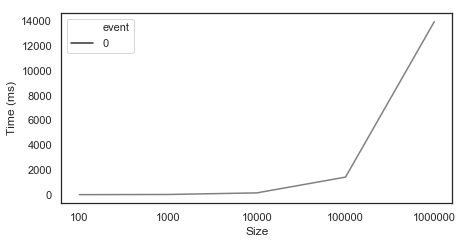
\includegraphics[width=0.4\textwidth]{pictures/introduction/timesize.png}
%	\vspace{-5mm}
%	\caption{The latency time for generating line-based visualization at each datasize.}
%	\vspace{-5mm}
%	\label{fig:rendering_time}
%\end{figure}




%The major challenges to design visual quality guaranteed sampling method are:
%(I) how to define visual quality theoretically? (II) how to guarantee the quality of the sampling-based visualization result?
%\TB{In this work, we study how to reduce the rendering time and preserve the visual quality for the large-scale trajectory visualization.}
%We extend the motivation of visualization-aware sampling to trajectory dataset and propose a novel sampling strategy, \textbf{v}isualization \textbf{a}ware \textbf{t}rajectory \textbf{s}ampling(VATS), that produces high-visual-quality line-based trajectory visualization at different zooming resolutions.
%%\QM{In this paper, we first proposed the visual fidelity loss function which effectively evaluates the visual loss of the sampling method. Then we minimize the loss function by transforming this problem to an optimization problem. Several solutions for efficiently solving the optimization problem are discussed.}
%We first format visual quality by defining the loss function between the visualization results of the whole dataset and sampled dataset.
%With the loss function, we analyze the hardness of the problem, and devise a visual quality guaranteed sampling algorithm for it.
%Figure~\ref{fig:compare} depicts an comparison among the ground truth,  uniform random sampling and our proposed method.
%With the same sampling set size($1\%$), the proposed method generates a higher-fidelity visualization and support the multi-resolution very well.
%At last, color encoding are applied to enhance the distribution of trajectories.
%
%\begin{figure}[t]
%	\centering
%	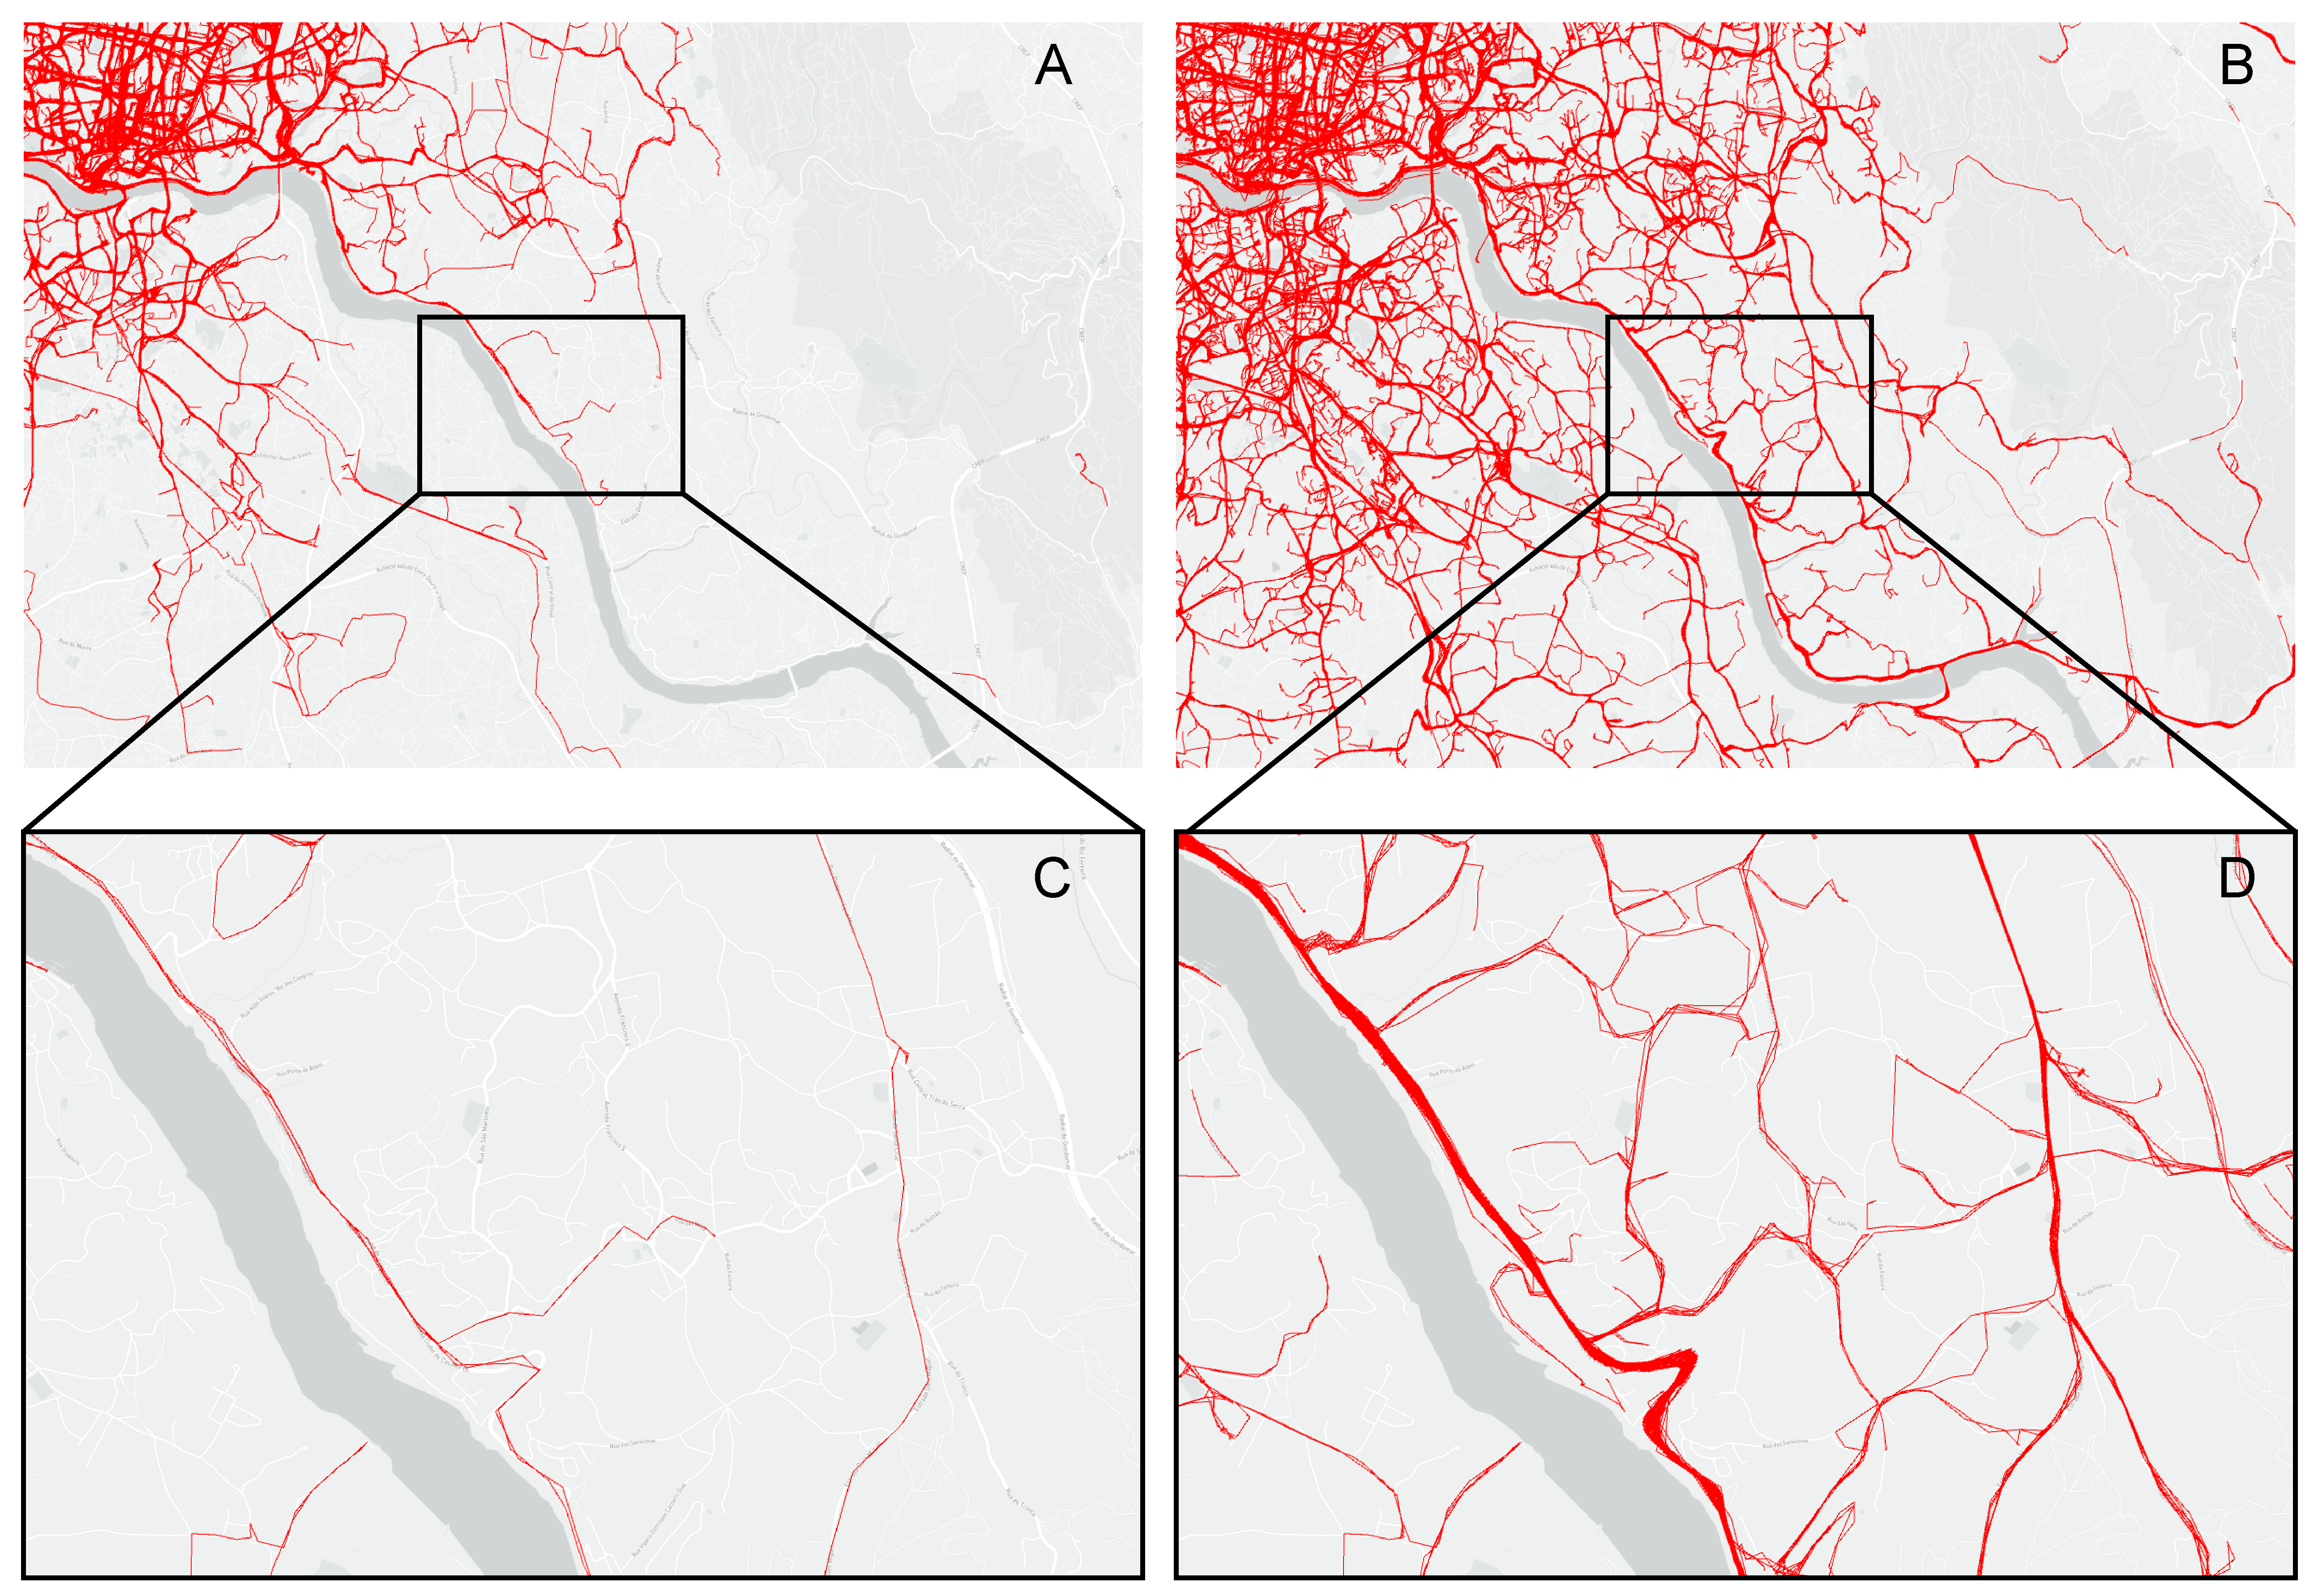
\includegraphics[width=0.44\textwidth]{pictures/introduction/effectiveness.pdf}
%	\vspace{-3mm}
%	\caption{Trajectory sampling generated by uniform random sampling(A,C) and VQGTS(B,D) at same sampling rate. In both high-level(A,B) and low level(C,D) view, our approach preserved more detail information about the trajectories especially for the sparse regions.}
%	\vspace{-5mm}
%	\label{fig:compare}
%\end{figure}
%

%
%
The remainder of this paper is organized as follows.
Section~\ref{sec:rel} discusses the related work.
Section~\ref{sec:pro} formulates our problem and analyze its hardness.
Section~\ref{sec:sol} provides an approximate solution for it, together with a suite of optimization techniques.
Section~\ref{sec:aa} proposes an advanced solution for our problem.
Section~\ref{sec:exp} elaborates our extensive experimental studies and our findings in detail.
Section~\ref{sec:con} concludes this work and highlights the promising future directions.

%\vspace{-2mm}
\section{Related work}
The most related techniques to our work include the visual analysis of trajectory dataset, the methodology of large data visualization and data sampling. 
\subsection{Trajectory analysis}
Trajectory, consisting of a sequence of spatial locations, is the most common form of the object movement. To support the understanding and analysis of the trajectory dataset, many visualization and visual analytics system are developed. The detailed summary of these work is presented in~\cite{chen2015survey}. These techniques can be classified into three categories according to visualization form: point-based visualization, line-based visualization and region-based visualization. 

The point-based visualization capture the basic spatial distribution of the passing points of the moving object\cite{}. Furthermore, many density-based methods such as the kernel density estimation(KDE) are applied based on the point-based visualization, by the sacrifice of the detail the information of trajectories, these methods alleviate the visual clutter caused by large amount of data. 
Furthermore, to be better applied in the city environment, advanced KDE techniques are developed to capture the moving patterns along the road networks~\cite{}. In the study of urban traffic, the point-based visualization can capture the hot regions, but unable to identify the movement of the individual case and reveal the moving information such as the direction and origin-destination ~\cite{chen2015survey}. Line-based techniques are the most commonly used visualization methods which present the trace of the movement as polylines, thus to preserve the continuous moving information~\cite{}. However, due the large amount of the trajectories, the line-based methods always cause serious visual clutter due to the cross of the polylines~\cite{}. To alleviate this problem, the clustering techniques are applied in the preprocessing step before visualization and then visualize the clusters by ribbon ~\cite{},  glyph~\cite{} or sankey diagrams~\cite{}. Moreover, advanced interaction techniques~\cite{}, sampling techniques~\cite{} and edge bundling techniques~\cite{zeng2019route} are also developed to better present the movement patterns. The region based techniques divide the whole region into sub-regions in advance and then visualize the traffic situation before the sub-regions. These methods visualize the macro-pattern very well by leveraging different aggregation techniques such as the administrative regions~\cite{}, uniform grid~\cite{} and spatial clustering results~\cite{}.


\subsection{Large data visualization}
Another topic related to our work is the large data visualization. The movement dataset, such as the urban traffic, always contains millions to billions of trajectories, which is challenge to analyze and visualize. Three methods are applied to support the visual analytics of large datasaet: interactive method, aggregation method and reduction method. All these methods aim to reduce the amount of the rendering items to support the efficient visualization. 

\QM{More discussion about the limitations}

\subsection{Data sampling techniques}
As we have discussed in the previous sections, the sampling methods reduce the data volume by directly selecting the representative items. Current advancing sampling techniques in the visualization domain are mostly designed for the scatter plot and aim to not only solve the overdrawing of the points but also try to preserve the information distribution of the data items. 
Some works design advanced sampling algorithms to preserve the meaningful data items according to the analyzing requirement such as the mulit-class data analysis~\cite{chen2014visual} and hierarchical exploration~\cite{}. Furthermore, to the usage of more visual channels of the points other than location such as color~\cite{chen2014visual}, size~\cite{woodruff1998constant} and opacity are discussed. 
Closely related to our work, Park et al.~\cite{park2016visualization} proposed the visualization-aware techniques for the scatter plot. They proposed visualization-inspired loss which effectively evaluates the visual loss of the sampling result and validates the proposed method based on three common visualization goals:  regression, density estimation and clustering. 

In comparison with the sampling techniques for scatter plot, the trajectory sampling is more challenging because of the complexity of the trajectories~\cite{pelekis2010unsupervised}. \QM{Most} of the existing trajectory sampling techniques cluster the trajectories first~\cite{pelekis2009clustering} and then select the most representative trajectories from each cluster, which highly depend on the distance calculation~\cite{pelekis2007similarity} and clustering algorithms. Some techniques further focus on the clustering and sampling of trajectory segments instead of the whole trajectories~\cite{panagiotakis2011segmentation}. 
\QM{None of these sampling techniques are proposed from the motivation visualization-aware...}
%\vspace{-2mm}
\section{Problem formulation}
%\\Visualizing a large collection of trajectories are used frequently in map service or smart city applications.
When exploring a large collection of trajectories, efficient and effective large-scale trajectory visualization is challenging in both academia and industry.
The reasons are (i) the size of trajectory data is very large (e.g., several GB in an hour),
and (ii) the limited rendering ability of existing commercial graphics device (e.g., XXX).
Sampling is a delta-facto solution for the problems with big data. The naive solutions such as uniform random sampling cannot generate acceptable because the serious visual information loss. In this section, we first define a loss function to evaluate the visual quality between the visualization results between whole dataset and sampled subset. Then we analyze the hardness of the problem and design algorithms for it.  
%A naive solution to employ sampling idea for large-scale trajectory visualization problem is randomly selecting several trajectories from the data set then visualize it by graphics device.
%However, the visualization result may be not acceptable by the user.
%In this work, we study the large-scale trajectory visualization problem.
%In particular, we focus on visual quality guaranteed sampling method for large trajectory data visualization.
%The major challenges to design visual quality guaranteed sampling method are:
%(I) how to define visual quality theoretically? (II) how to guarantee the quality of the sampling-based visualization result?
%In this work, we first formate visual quality by defining the loss function between the visualization results of the whole dataset and sampled dataset.
%\\With the loss function, we analyze the hardness of the problem, and devise a visual quality guaranteed sampling algorithm for it.

\subsection{Problem description}
\begin{problem}[Sampling-based trajectory visualization problem]\label{prob:def}
Given a large-scale trajectory dataset $\D$ and an integer $k$,
the trajectory visualization problem is selecting a subset of trajectories $\oR \subseteq \D$, such that loss function $loss(\oR,\D)$ is minimized.
\end{problem}

From the user’s perspective, there are many ways to define the loss function $loss$ between the visualization result qualities of the sampled subset $\oR$ and the whole dataset $\D$.
For example, \cite{park2016visualization} defined point-based loss function for very large scatter points visualization.
However, it is not applicable for trajectory data visualization.
In order to address that, we propose an novel loss function for trajectory visualization problem.

Intuitively, the visual quality difference between the visualization results of two trajectory datasets depends on the user specified visualization level of details (a.k.a., LOD).
Given an empty canvas (e.g., displaying device) with a user specified level of details, 
the visualization process is rendering the trajectories into canvas with the given level of details (e.g., the number of pixels in each row and each column).
Considering a trajectory data set $\D$ and a subset of trajectories $\oR \subseteq \D$,
The visual quality loss between $\oR$ and $\D$ is defining as the different pixels of the visualization results about $\oR$ and $\D$ in the canvas with specified LOD.
We then define the loss function of sampling-based trajectory visualization problem as $loss(\D, \oR) = \frac{\V(\D) - \V(\oR)}{\V(\D)}$,
where $\V()$ measures the number of rendered pixels in the canvas of a given trajectory dataset.

Given a trajectory data set $\D$ and an integer $k$,  our research objective is finding subset $\oR$, such that  the visualization quality loss function $loss(\D, \oR)$ is minimized,
i.e.,
$$ \min_{\oR \subseteq \D, |\oR| = k}  loss(\D, \oR) =  \frac{\V(\D) - \V(\oR)}{\V(\D)}. $$ %\\ %\nonumber


%  \Leftrightarrow  & \min_{\oR \subseteq \D, |\oR| = k}  \V(\D) - \V(\oR) \\ \nonumber
%  \Leftrightarrow  & \min_{\oR \subseteq \D, |\oR| = k}  \sum_{\forall \D_i \in \D} \V(\D_i) - \V(\oR)
%Intuitively, the visualization quality from user's perspective highly depends on the resolution of displaying device,
%e.g., the number of distinct pixels in each dimension that can be displayed.

%Given a high resolution displaying device, data objects set $\D$, and a subset of data objects $\oR \subseteq \D$.
%The visualization quality loss between $\oR$ and $\D$ is defining as the different pixels of the visualization results of $\oR$ and $\D$ in the given display device.
%Given a trajectory data set $\D$ and an integer $k$,  our research objective is selecting a sized-$k$ subset of trajectories which minimize
%the visualization quality loss function $loss(\D, \oR)$.
%Formally, the loss function is defined as $loss(\D, \oR) = \V(\D) - \V(\oR)$.



\subsection{Hardness analysis}
In real-world applications, the pixels in canvas will be rendered by different colors according to the specified visualization scheme.
For the sake of presentation, we analyze the hardness of our research objective with a simple render manner of visualization result.
In particular, for each pixel in the canvas, it will be rendered if there is a trajectory pass through it, otherwise it will not be rendered.
Suppose each pixel in the canvas has an unique id, let $\U$ be the universal set of all pixels in the canvas
For each trajectory $\D_i \in \D$, it consists of a set of pixels in the canvas, e.g., it is a subset of $\U$.
Thus, the subset $\oR$ also is a subset of $\U$ as $\oR = \cup_{\oR_i \in \oR} \oR_i$.

Our research objective is minimizing loss function $loss(\D, \oR) =  \frac{\V(\D) - \V(\oR)}{\V(\D)}$.
Obviously, the visualization result of $\D$ is a constant value, denotes as $\mathsf{C}$.
Our research objective of Problem~\ref{prob:def} can be transformed as follows:
\begin{align}\label{eqn:obj2} \nonumber
\text{Objective}: & \min_{\oR \subseteq \D, |\oR| = k}  \frac{\V(\D) - \V(\oR)}{\V(\D)} \\ \nonumber
& \Leftrightarrow \min_{\oR \subseteq \D, |\oR| = k}  \frac{\mathsf{C} - \V(\oR)}{\mathsf{C}} \\ \nonumber
& \Leftrightarrow \max_{\oR \subseteq \D, |\oR| = k}  \cup_{\oR_i \in \oR} \oR_i
\end{align}

It is equivalent to select sized-$k$ trajectory set $\oR$ from $\D$ which $\cup_{\oR_i \in \oR} \oR_i$ is maximized.

It is a typical set cover maximization problem\footnote{\url{https://en.wikipedia.org/wiki/Maximum_coverage_problem}}, which is a well-known NP-hard problem in literature.

%It is equivalent to select sized-$k$ trajectory set $\oR$ from $\D$ which $\cup_{\oR_i \in \oR} \oR_i$ is maximized.
%It is a NP-hard problem as we proved in Lemma~\ref{lem:np}.

%\begin{lemma}[NP hard]~\label{lem:np}
%Given a trajectory dataset $\D$ and an integer $k$, 
%The sampling-based trajectory visualization problem (see Problem~\ref{prob:def}) is NP-hard.
%\end{lemma}

%We omit the proof of Lemma~\ref{lem:np} as it is a typical set cover maximization problem\footnote{\url{https://en.wikipedia.org/wiki/Maximum_coverage_problem}}, which is a well-known NP-hard problem in literature.


%\vspace{-2mm}
\section{Visual Fidelity Guaranteed Sampling Approach}\label{sec:sol}
Due to the hardness of the Problem~\ref{prob:def}, we first introduce a straight-forward solution (i.e., uniform random sampling) for it in Section~\ref{sec:random}.
Then, we propose a visual fidelity guaranteed sampling approach in Section~\ref{sec:greedy}.
Last, we devise several optimizations to improve the efficiency and effectiveness of our proposal in Section~\ref{sec:opt}.


\subsection{Uniform Random Sampling Algorithm}\label{sec:random}
The straight forward solution for Problem~\ref{prob:def} is uniform random sampling $\rand$.
As the pseudocode in Algorithm~\ref{alg:rand} shown, it selects $k$ trajectories from $\D$ randomly, which stores in $\oR$,
then render these selected trajectories in $\oR$ as the visualization result.

\begin{algorithm}
    \caption{$\rand(\D,k=\alpha |\D|)$} \label{alg:rand}
    \begin{algorithmic}[1]
    \State Initialize result set $\oR \leftarrow \emptyset$
    \While{$|\oR| < k$}
        \State $tmp \leftarrow \mathsf{RandomSampling(\D-\oR)}$
        \State $\oR \leftarrow \oR \cup \{ tmp \}$
    \EndWhile
    \State Return $\oR$
    \end{algorithmic}

\end{algorithm}



Obviously, the uniform random sampling algorithm has good performance.
However, it does not provide any guarantee on the visual fidelity of the sampled result set.


%Trajectory data $\D$\cite{xxx} consists of almost 10K trajectories which collected by Didi company.
%The visualization result of the whole dataset $\D$ is illustrated in Figure~\ref{fig:demo}(b).
%Figure~\ref{fig:demo}(b) shows the visualization result of uniform random sampling result of $\D$ with $k=100$.
%The difference between the visualization results in Figures~\ref{fig:demo}(a) and (b) are obvious from user's perspective.

%\begin{figure}
% \centering
% \small
% \begin{tabular}{cc}
%   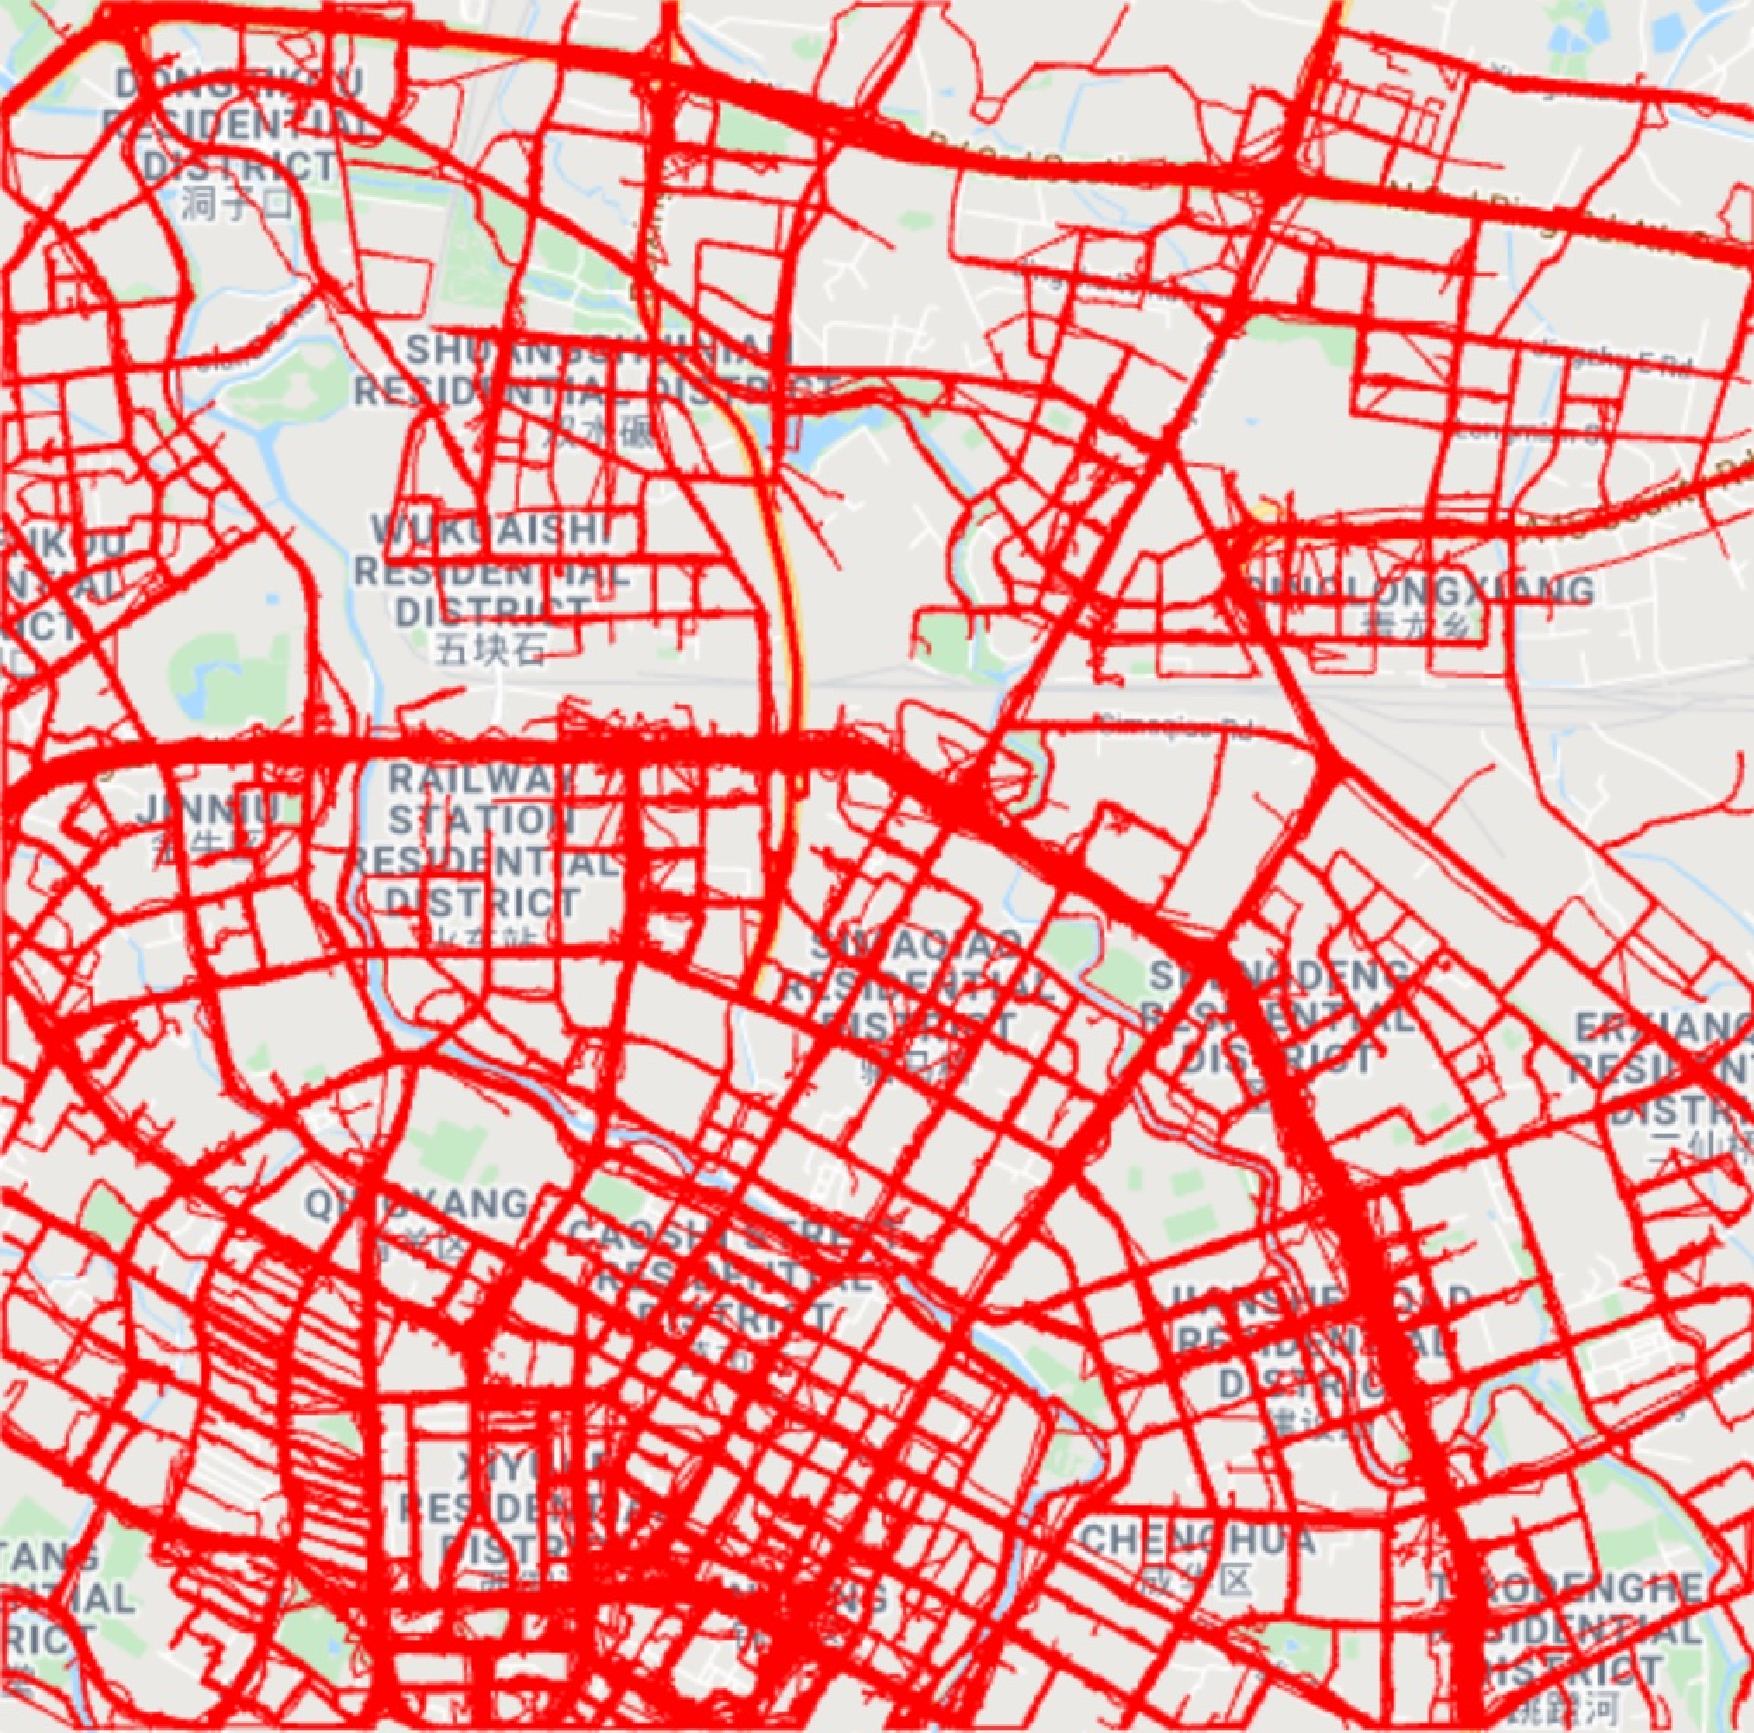
\includegraphics[width=0.45\columnwidth]{chengdu_total}
%   &
%   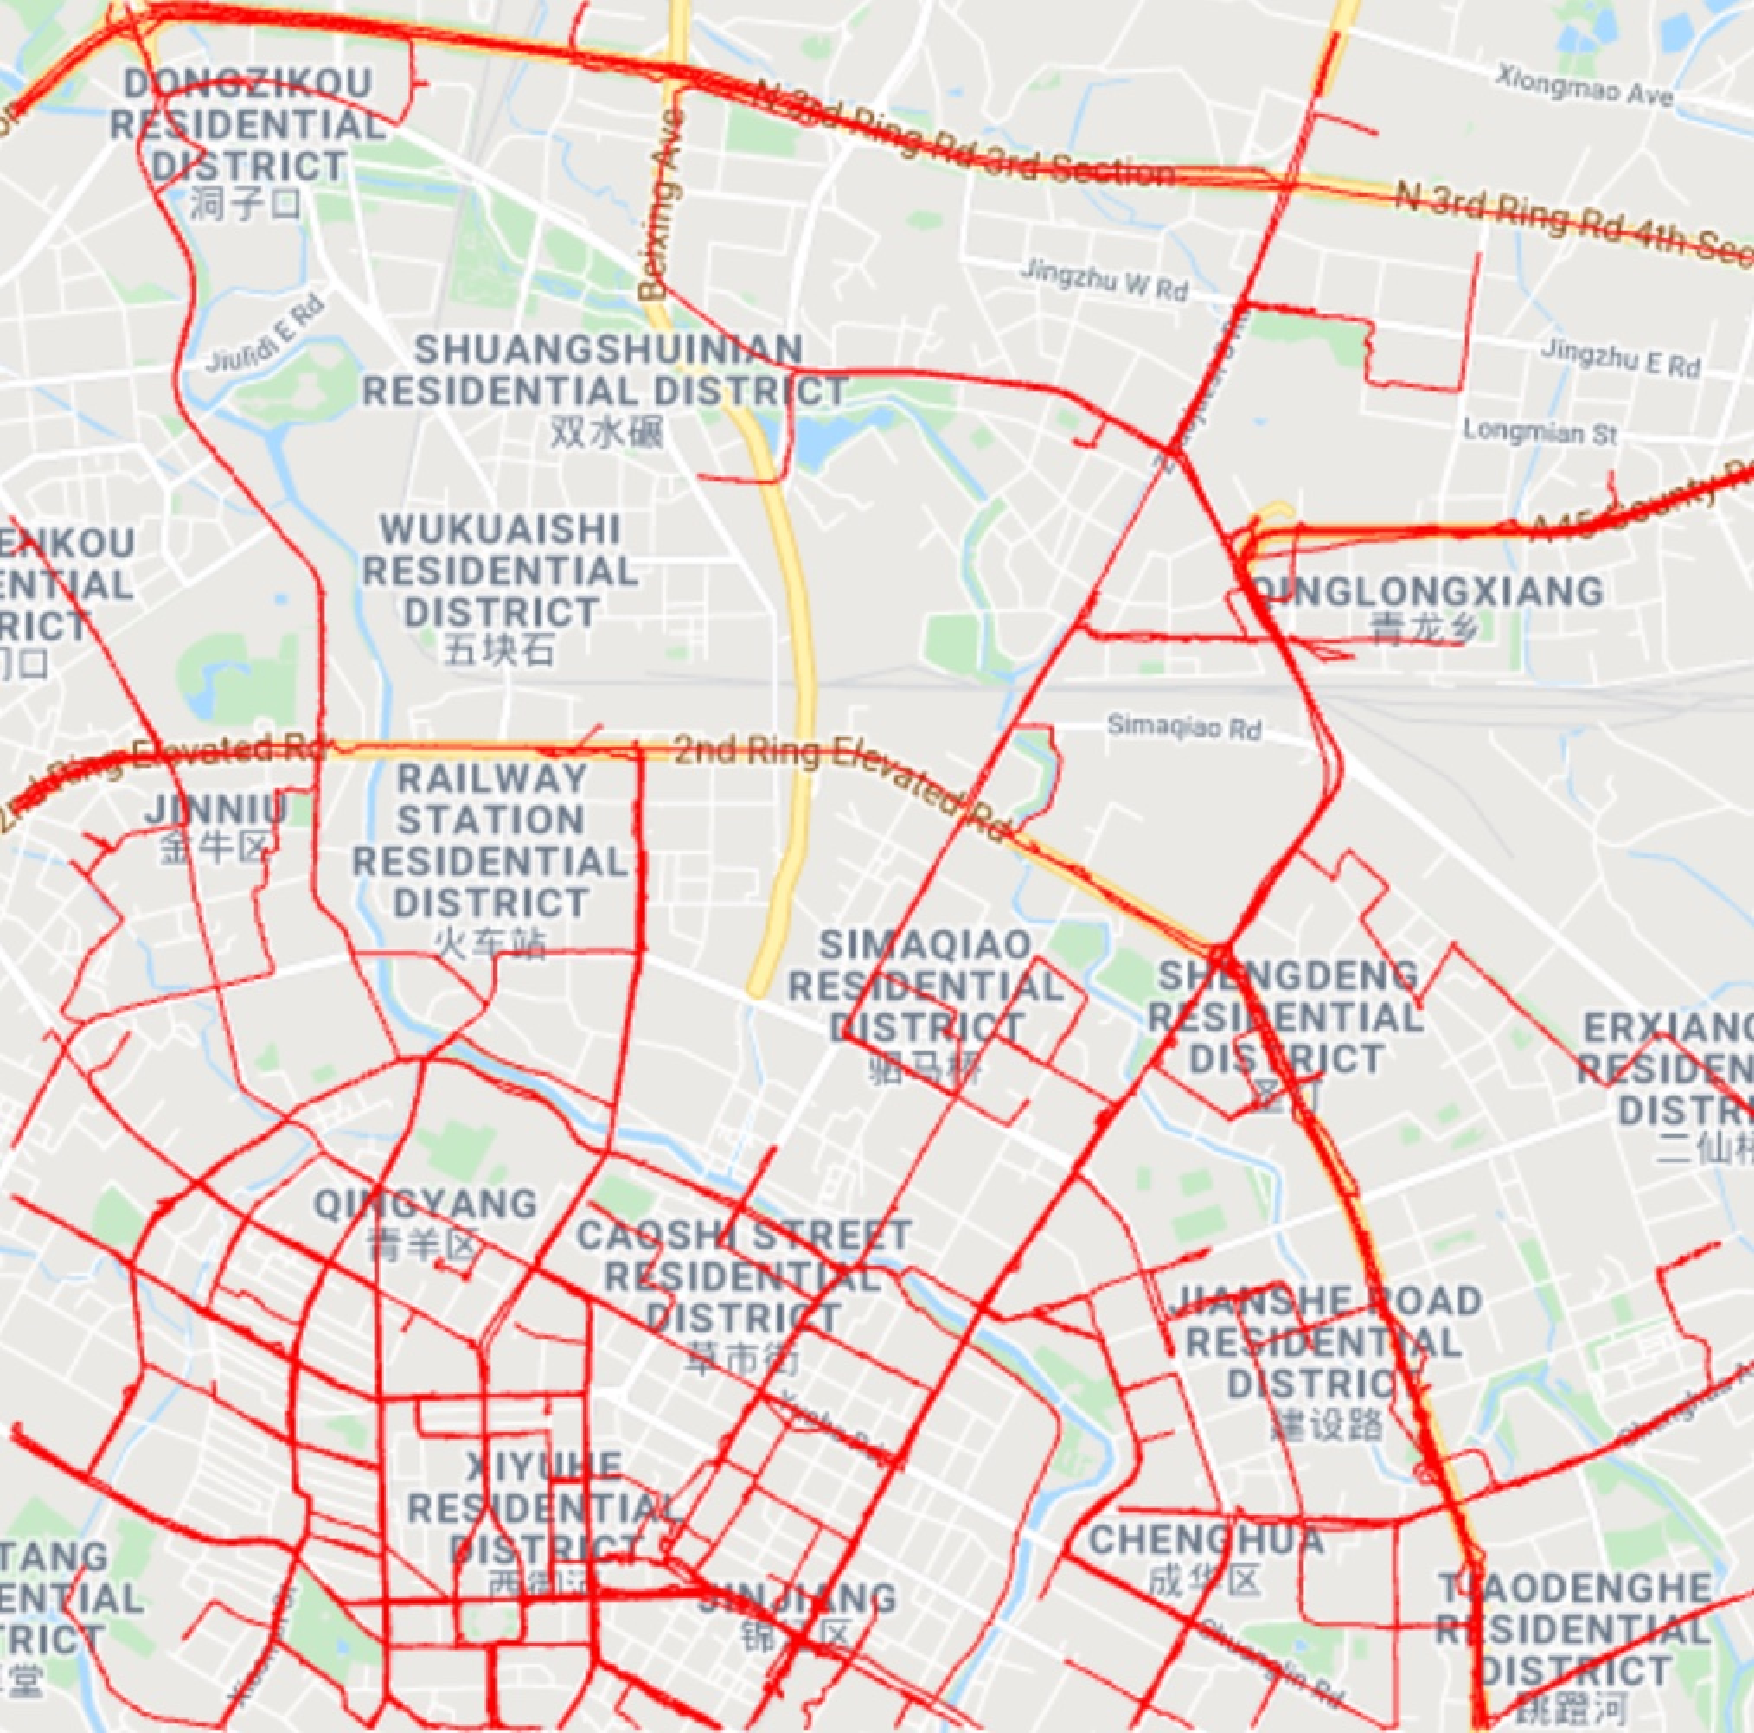
\includegraphics[width=0.45\columnwidth]{chengdu_sampling}
%   \\
%   (a) Dataset $\D$
%   &
%   (b) Uniform sampling $\oR$
% \end{tabular}
% \caption{Visualization results of trajectory set in Chengdu}
% \label{fig:demo}
%\end{figure}

\subsection{Visual Fidelity Guaranteed Sampling Algorithm}\label{sec:greedy}
In this section, we present our visual fidelity guaranteed sampling algorithm for Problem~\ref{prob:def}.
We start our presentation by elaborating the correlation between visual fidelity of sampled set $\oR$ and user zoom level.
For a given sampled set $\oR \subseteq \D$, it has different visual fidelity loss values at different user zoom levels.
The reason is the resolutions of $\oR$'s visualized result are different at different zoom levels.
%The reason is the pixel size will be updated at different zoom level.
%\QM{The reason is the map are of the same canvas region will be updated at different zoom level.}
For example, Google map~\cite{googlemap} provides zoom levels range from 0 to 20,
where level 0 is the lowest level (e.g., the whole world), level 20 is the highest level (e.g., individual building, if available).
In order to devise a zoom level oblivious visualization for sampled dataset $\oR$,
we use the highest zoom level to define the size of each pixel in the canvas in our problem.
It means for each trajectory $t_i \in \D$, it is a set of pixels in the canvas at the highest zoom level.

The visual fidelity guaranteed sampling algorithm employs greedy paradigm.
In particular, it finds the trajectory $tmp$ in $\D$ which maximize the result set of $|\oR \cup tmp|$ at each iteration, as Line~\ref{line:max} shown in Algorithm~\ref{alg:greedy}.
It terminates after $k=\alpha |\D|$ iterations and returns $\oR$ as result set for rendering.

\vspace{-2mm}
\begin{algorithm}
    \caption{$\vats(\D,k=\alpha |\D|)$} \label{alg:greedy}
    \begin{algorithmic}[1]
    \State Initialize result set $\oR \leftarrow \emptyset$
    \While{$|\oR| < k$}
        \State $tmp \leftarrow argmax_{t_i \in \D} |\oR \cup t_i|$ \label{line:max}
        \State $\oR \leftarrow \oR \cup \{ tmp \}$
    \EndWhile
    \State Return $\oR$
    \end{algorithmic}
\end{algorithm}
\vspace{-2mm}

Interestingly, Algorithm~\ref{alg:greedy} offers theoretical visual fidelity guarantee of the returning result $\oR$, as proved in Theorem~\ref{the:ratio}.

\begin{theorem}~\label{the:ratio}
Algorithm~\ref{alg:greedy} provides $1-(1-1/k)^k \geq (1-1/e) \approx 0.632$ approximation result for large-scale trajectory visualization problem (i.e., Problem~\ref{prob:def}).
\end{theorem}

\begin{proof}
The optimal solution of Problem~\ref{prob:def} covers $OPT$ pixels in $k$ iterations.
Let $a_i$ be the number of newly covered pixels at the $i$-th iteration, $b_i$ is the total number of covered pixels up to the $i$-th iteration (i.e., $b_i = \sum_{j=1}^{i}a_i$),
and $c_i$ be the uncovered pixels after $i$-th iteration (i.e., $c_i = OPT-b_i$).
According to greedy paradigm, we can conclude the number of newly covered pixels at the $(i+1)$-th iteration is always greater than or equal to $\frac{1}{k}$ of the number of uncovered pixels after the $i$-th iteration, i.e., $a_{i+1} \geq \frac{c_i}{k}$.
We prove Theorem~\ref{the:ratio} by proving $c_{i+1} \leq (1-1/k)^{i+1} \cdot OPT$.
It holds $c_1 \leq (1-1/k) \cdot OPT$ as follows.
\begin{align} \nonumber
& a_1 \geq c_0 \cdot 1/k = 1/k \cdot OPT \text{~~~as we concluded~~~} a_{i+1} \geq \frac{c_i}{k}\\ \nonumber
 \Leftrightarrow  & b_1 \geq 1/k \cdot OPT  \Leftrightarrow  -b_1 \leq - 1/k \cdot OPT  \text{~~~as~~~} a_1 = b_1\\ \nonumber
 \Leftrightarrow & OPT - b_ 1 \leq OPT - 1/k \cdot OPT  \Leftrightarrow  c_1 \leq (1-1/k) \cdot OPT
\end{align}
For inductive hypothesis assume $c_{i} \leq (1-1/k)^i \cdot OPT$. Thus,
\begin{align} \nonumber
& c_{i+1} = c_i - a_{i+1} \leq c_i - c_i/k = (1-1/k) \cdot c_i = (1-1/k)^{i+1} \cdot OPT
\end{align}

Hence, it holds $c_k \leq (1-1/k)^{k} \cdot OPT$.
It is equivalent to $b_k \geq (1 - (1-1/k)^{k}) \cdot OPT \geq (1-1/e) \cdot OPT \approx 0.632 \cdot OPT$.
\end{proof}


\subsection{Optimization Techniques}\label{sec:opt}
With the above analysis, Algorithm~\ref{alg:greedy} ($\vats$) provides a visual fidelity guaranteed sampling algorithm for large-scale trajectory data visualization problem.
However, it is inefficient for (very) large trajectory dataset (e.g., millions of trajectories) as the time complexity analyzed in the following Lemma~\ref{lem:cost}.

\begin{lemma}[Time Complexity]~\label{lem:cost}
Given trajectory dataset $\D$ and an integer $k = \alpha |\D|$, the time complexity of Algorithm~\ref{alg:greedy} is $O(\alpha \cdot m \cdot |\D|^2)$, where $m$ is the maximum length of all trajectories in dataset $\D$.
\end{lemma}

\begin{proof}
At each iteration ($k = \alpha |\D|$ iterations in total),
it computes the uncovered pixels of each trajectory in dataset $\D$ with $O(m)$ cost.
The dataset $\D$ has $O(|D|)$ trajectories.
Thus, the total cost is $O(k \cdot m \cdot |\D|)=O(\alpha \cdot m \cdot |\D|^2)$.
\end{proof}

\stitle{Example} Given \pt{} trajectory dataset, it has 2.39 millions of taxi trajectories, the maximum length in it is 3,490.
It takes 413.6 seconds to return a subset $\oR$ with sampling rate $0.1\%$.
Obviously, it is impractical for interactive trajectory explorations.

Due to the inefficient of our visual fidelity guaranteed sampling approach in Algorithm~\ref{alg:greedy},
we then devise performance optimizations to accelerate its running time.
The core idea is utilizing the submodularity of the covered pixels of result set $\oR$, as shown in Lemma~\ref{lem:submodular}.

\begin{lemma}[Submodularity]\label{lem:submodular}
Suppose the contribution of trajectory $t$ to the result set $\oR$ is $\Delta(\oR, t) = |\oR \cup t| - |\oR|$.
Given a trajectory $t$ and two result sets $\oR,\oR^{'}$, where $\oR \subset \oR^{'}$ and $t \notin \oR$,
it holds $ \Delta(\oR, t) \geq \Delta(\oR^{'}, t)$.
\end{lemma}

\begin{proof}
The contribution value of trajectory $t$ to a given result set $\oR$ (e.g., $\Delta(\oR, t) = |\oR \cup t| - |\oR|$) is the new covered pixels of $t$ w.r.t. result set $\oR$, i.e., $|t| - |\oR \cap t|$.
It holds $t \cap \oR \subseteq  t \cap \oR^{'}$ as $\oR^{'}$ is a superset of $\oR$.
Thus, we have $|t| - |t \cap \oR| \geq |t| - |t \cap \oR^{'}|$.
Hence, it holds $\Delta(\oR, t) = |\oR \cup t| - |\oR| \geq |\oR^{'} \cup t| - |\oR^{'}|= \Delta(\oR^{'}, t)$.
\end{proof}

\begin{figure}
 \centering
 \small
 \begin{tabular}{cc}
   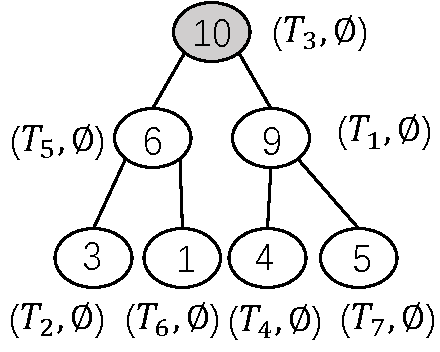
\includegraphics[width=0.35\columnwidth]{1st}
   &
   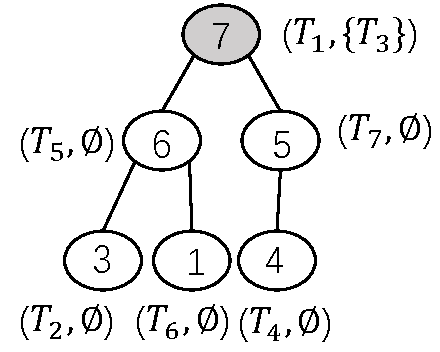
\includegraphics[width=0.35\columnwidth]{2nd}
   \\
   (A) 1st iteration
   &
   (B) 2nd iteration
 \end{tabular}
 \vspace{-3mm}
 \caption{An illustration of lazy computing manner via Lemma~\ref{lem:submodular}} \label{fig:heap}
 \vspace{-6mm}
\end{figure}


With the help of submodularity in Lemma~\ref{lem:submodular}, it reduces many unnecessary trajectory contribution value computations.
In particular, we maintains a max-heap for the number of uncovered pixels of each trajectory,
we employ lazy computing manner, i.e., only compute the contributions of a given trajectory when it is necessary.
Fig.~\ref{fig:heap}(a) shows a tiny max-heap example about the numbers of uncovered pixels of each trajectory from $t_1$ to $t_7$ with result set $\oR=\emptyset$.
At the 1st iteration, the root node of the max-heap will be selected, i.e., $t_3$ in Fig.~\ref{fig:heap}(A).
At the 2nd iteration, the number of uncovered pixels of the root node $t_1$ is updated to 7 w.r.t. result set $\oR = \{t_3 \}$ (see gray node at Fig.~\ref{fig:heap}(B)).
Then $t_1$ will be selected at the 2nd iteration without computing the number of uncovered pixels in other trajectories, i.e., all white nodes at Fig.~\ref{fig:heap}(B).
The reason is their contributions will be less than 7 via the submodularity shown in Lemma~\ref{lem:submodular}.

%In summary, the number of uncovered pixels in each trajectory will only be computed with the latest result set $\oR$ when it is necessary in the lazy computing manner,
%e.g., only $t_1$ will be updated at the 2nd iteration in Figure~\ref{fig:heap}.
%It reduces many unnecessary computations through the lazy updating manner, e.g., all white nodes did not update at the 2nd iteration in the above example.

%We then analyze the time complexity of Algorithm~\ref{alg:greedy} with lazy computing manner in Theorem~\ref{lem:lazy}.
%
%\begin{lemma}[Optimized Time Complexity]~\label{lem:lazy}
%Given trajectory dataset $\D$ and an integer $k= \alpha |\D|$, the time complexity of Algorithm~\ref{alg:greedy} with lazy computing manner is $O(\alpha \cdot m \cdot x |\D| \log |\D|)$, where $x$ is the number of contribution computations among all $k$ iterations and $x \ll |\D|$.
%\end{lemma}
%
%\begin{proof}
%It first takes $O(|\D|)$ time to construct the max-heap~\cite{cormen2009introduction}.
%It incurs $O( m \cdot x \log |\D|)$ cost to select the trajectory with maximum uncovered pixels at each iteration ($k$ iterations in total).
%Hence, the overall cost is $O(|\D| + k \cdot m \cdot t \log |\D|)$.
%\end{proof}
The performance of Algorithm~\ref{alg:greedy} is improved significantly as we only compute its contribution values when it is necessary.
To exemplify, Algorithm~\ref{alg:greedy} costs 413.6 seconds to return the results with sampling rate $0.1\%$ \pt{} taxi trajectory dataset.
However, it only needs 1.2 seconds in our performance optimized $\vats$.



\begin{figure}[t]
	\centering
	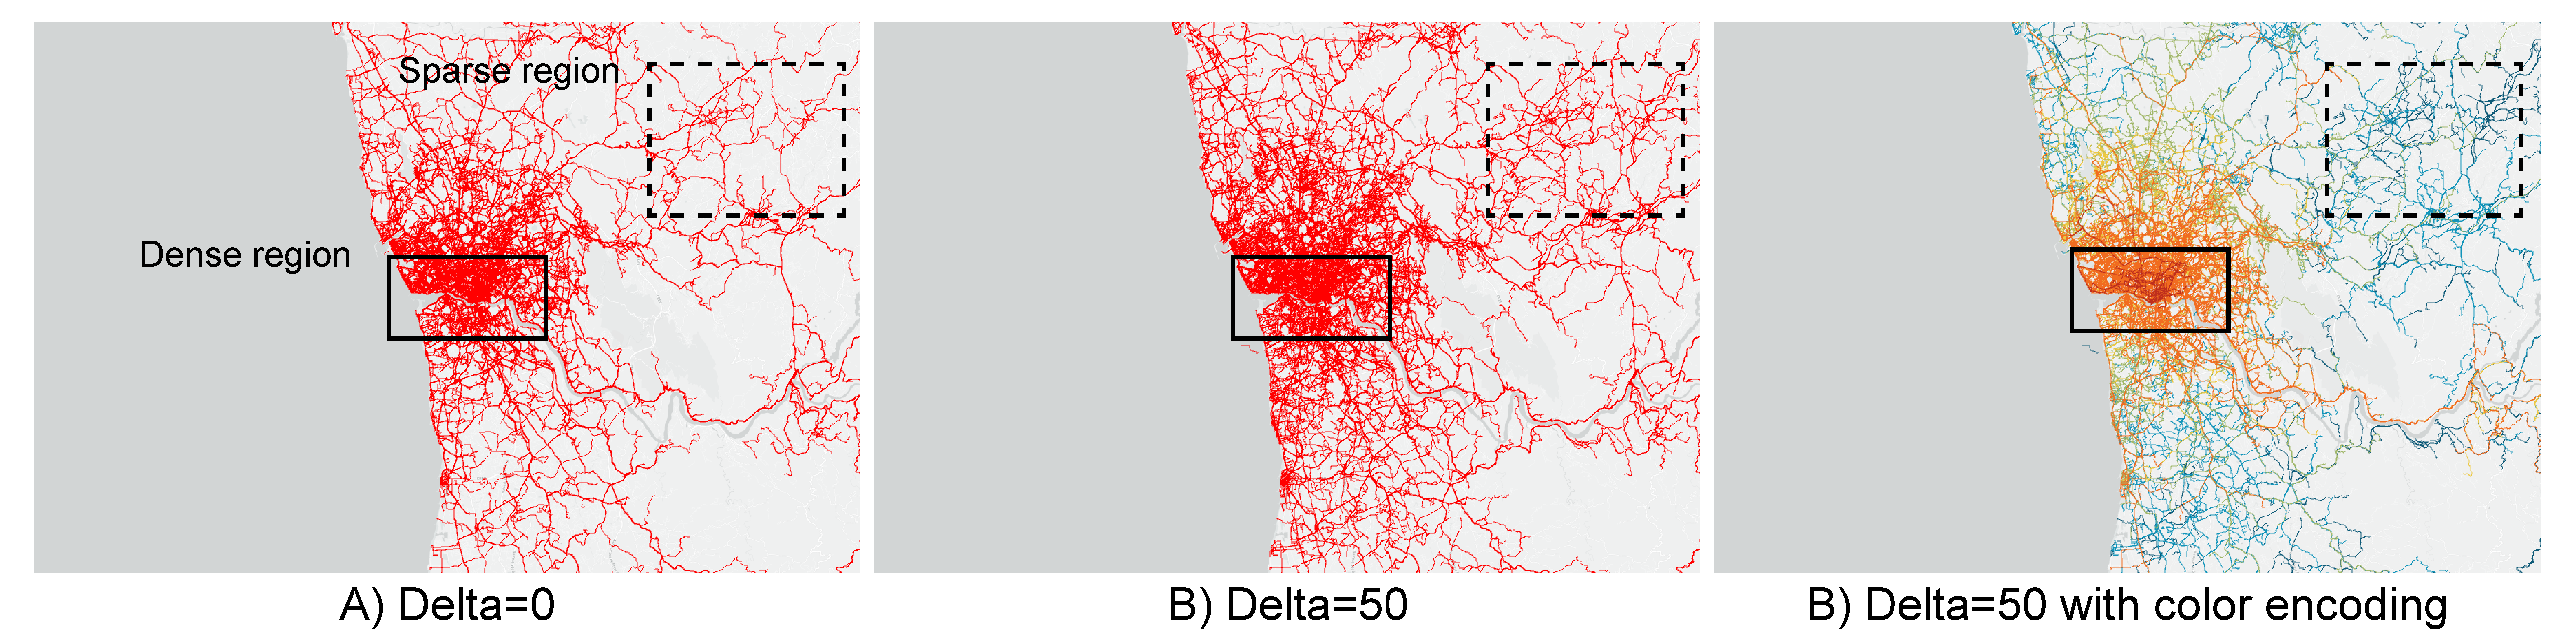
\includegraphics[width=0.48\textwidth]{pictures/problemsolveing/delta_motivation.pdf}
	\vspace{-3mm}
	\caption{Advance Approach $\avats$ with \pt{} trajectory dataset, sampling rate is $0.5\%$: (A) $\vats{}$, (B) $\avats$, and (C) $\cavats$}
	\label{fig:delta}
	 \vspace{-3mm}
\end{figure}


%https://developers.google.com/maps/documentation/maps-static/dev-guide#Zoomlevels

%\begin{figure}[t]
%	\centering
%	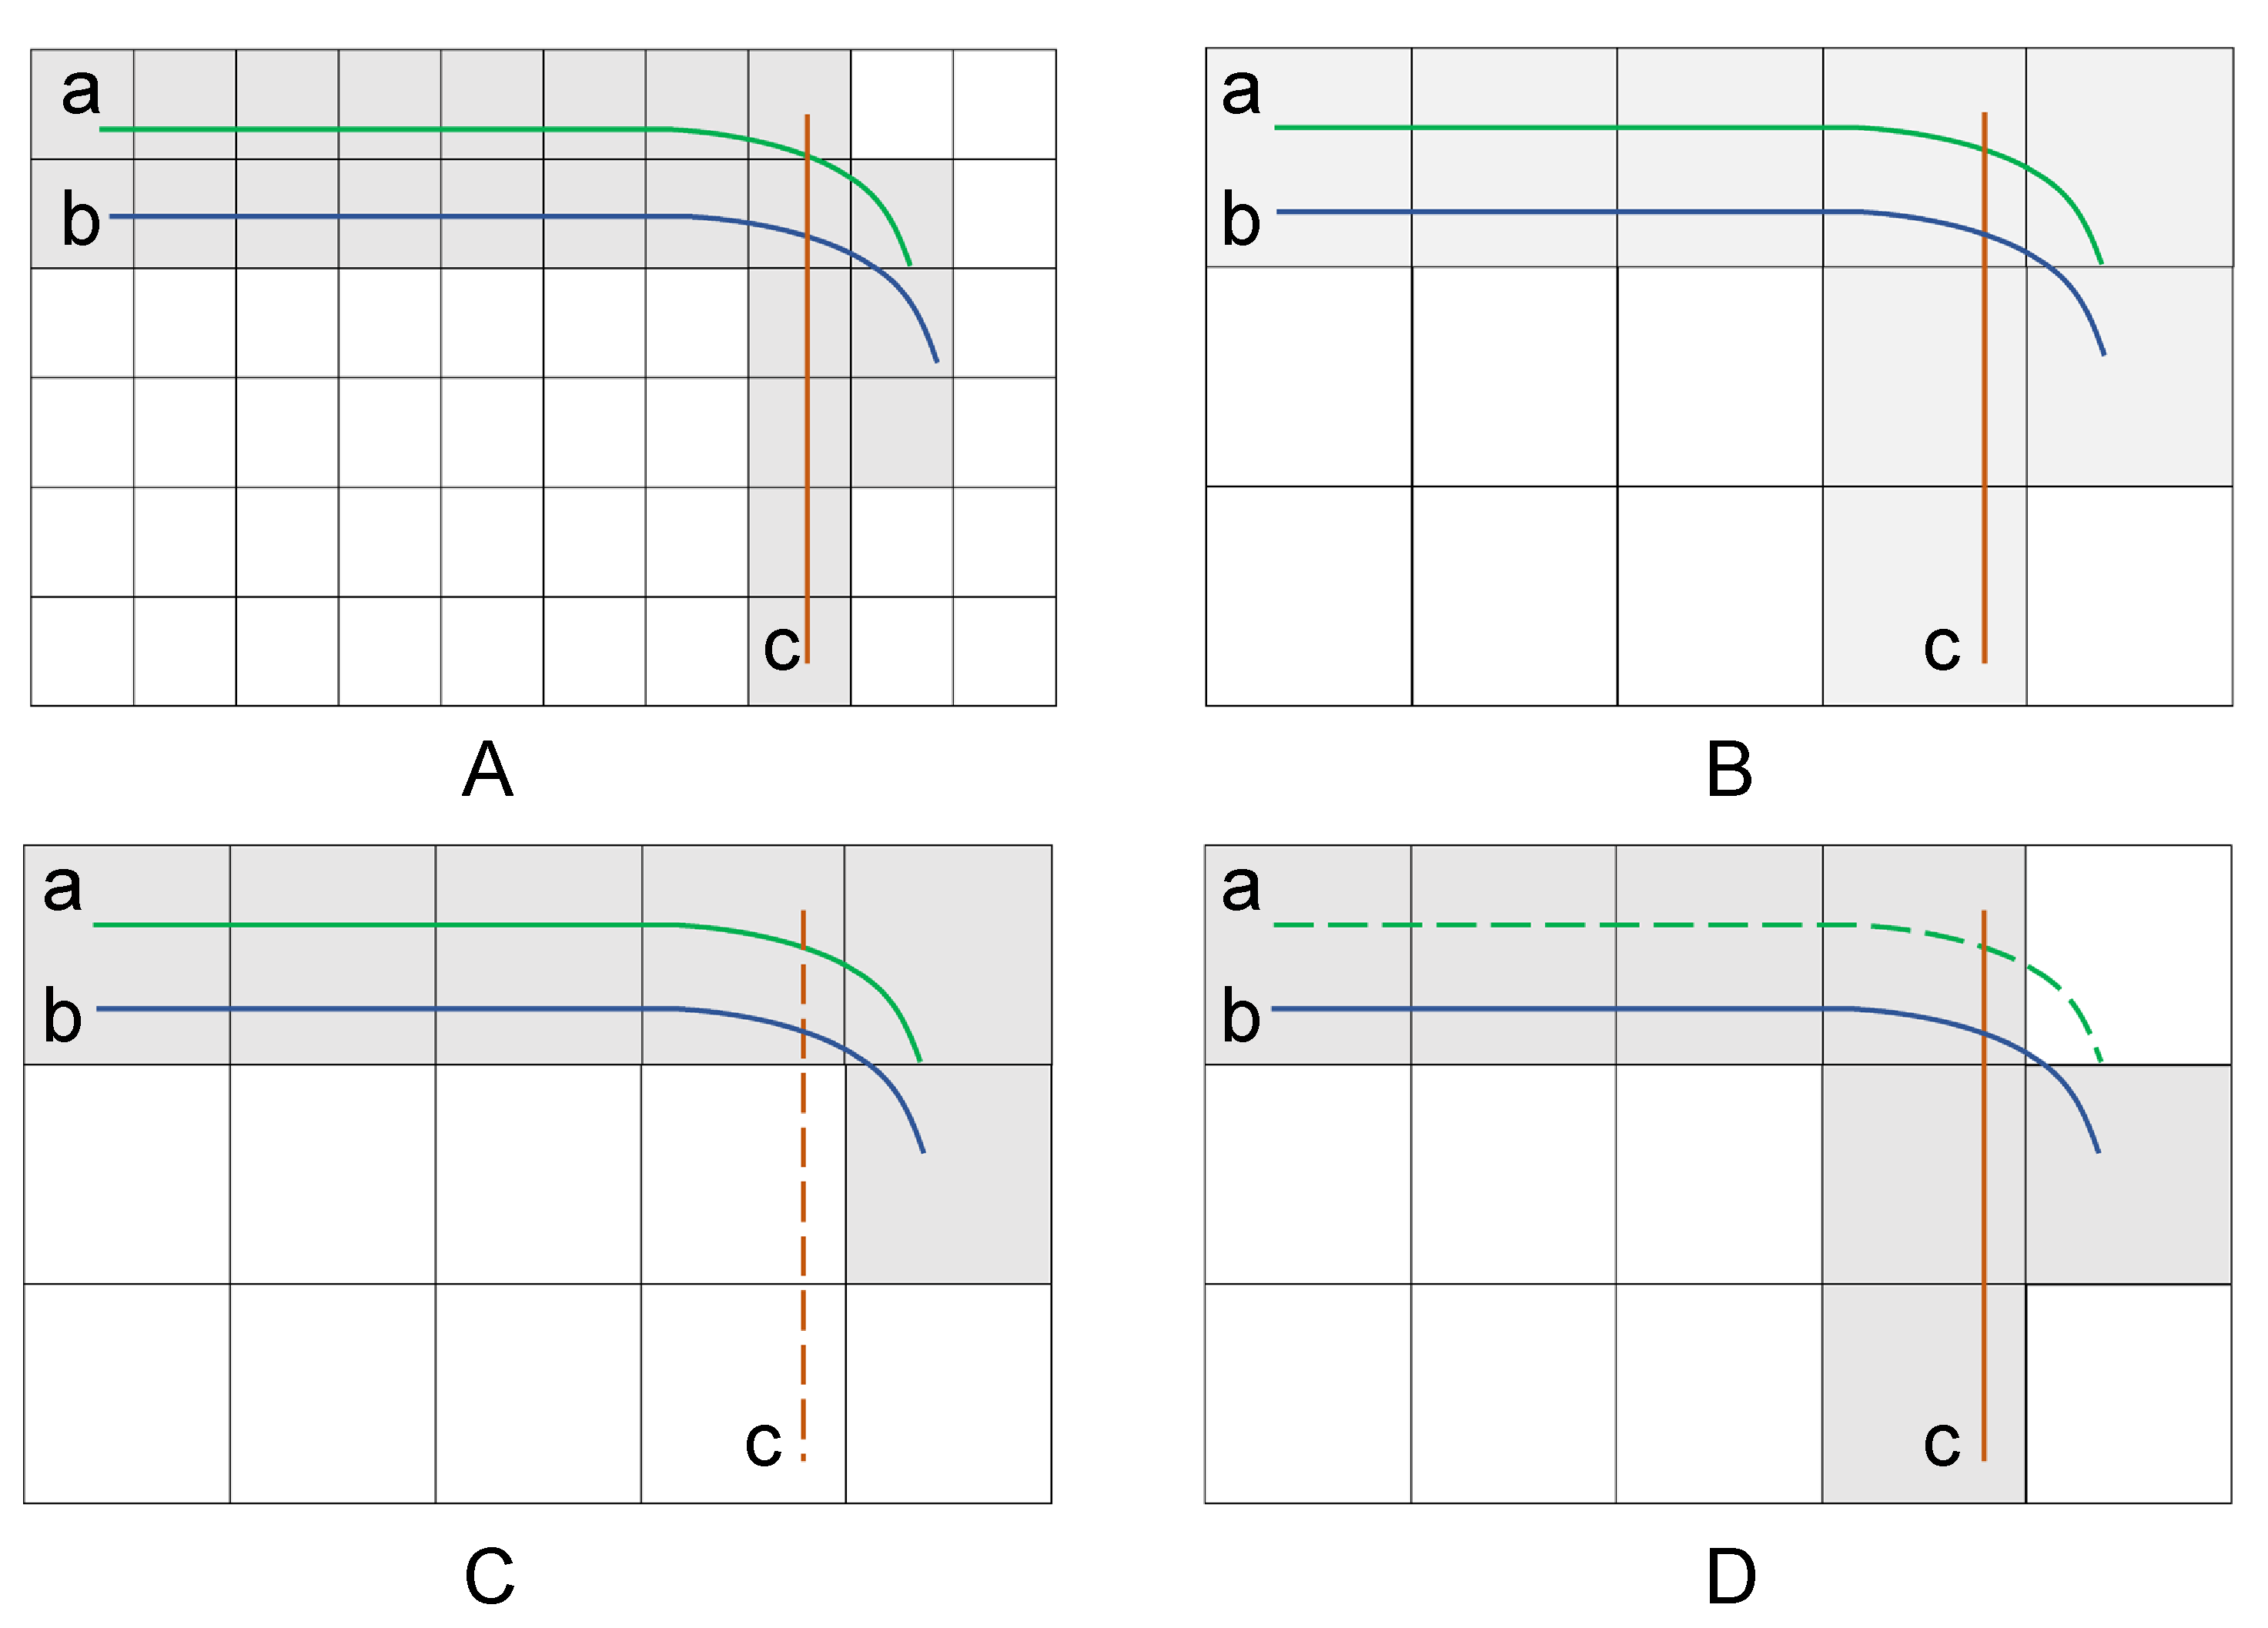
\includegraphics[width=0.4\textwidth]{pictures/problemsolveing/one_to_many.pdf}
%	\vspace{-5mm}
%	\caption{Resolution inconsistency}
%	\vspace{-5mm}
%	\label{fig:one_to_many}
%\end{figure}

%\subsection{One-to-many strategy}~\label{sec:one_to_many}
%Since we detect the covered pixels in the highest level, two trajectories may be very close to each other but share very few pixels, which will lead to more information loss in the low zoom view as figure~\ref{fig:one_to_many}.
%We next elaborate a ``one-to-many'' strategy to further optimize the visual quality of our proposed technique.
%Recalling we use the highest zoom level to define the pixel size in the canvas.
%Thus, our visual quality guaranteed sampling algorithm is zoom-level oblivious, e.g., it guarantees the visual quality of result set $\oR$ at every zoom level.
%However, users always do not use/need the highest zoom level in visualization applications.
%For example, Google map shows city and streets at zoom level 1 and 15, respectively~\footnote{\url{https://developers.google.com/maps/documentation/}}.
%Motivated by the above observation, we devise ``one-to-many'' strategy by introducing a visual tolerance parameter $\delta$ to optimize the visual quality for users.
%Specifically, suppose the pixel with location $(x,y)$ in canvas is covered by result set $\oR$,
%the ``one-to-many'' strategy will ignore all the pixels around $(x,y)$ within $\delta$ offset distance, i.e., all pixels from $(x-\delta, y-\delta)$ to $(x+\delta, y+\delta)$ will be skipped.
%We will demonstrate the effectiveness of the visual tolerance $\delta$ in experimental evaluations.
%
%%https://developers.google.com/maps/documentation/maps-static/dev-guide#Zoomlevels
%\begin{figure}[t]
%	\centering
%	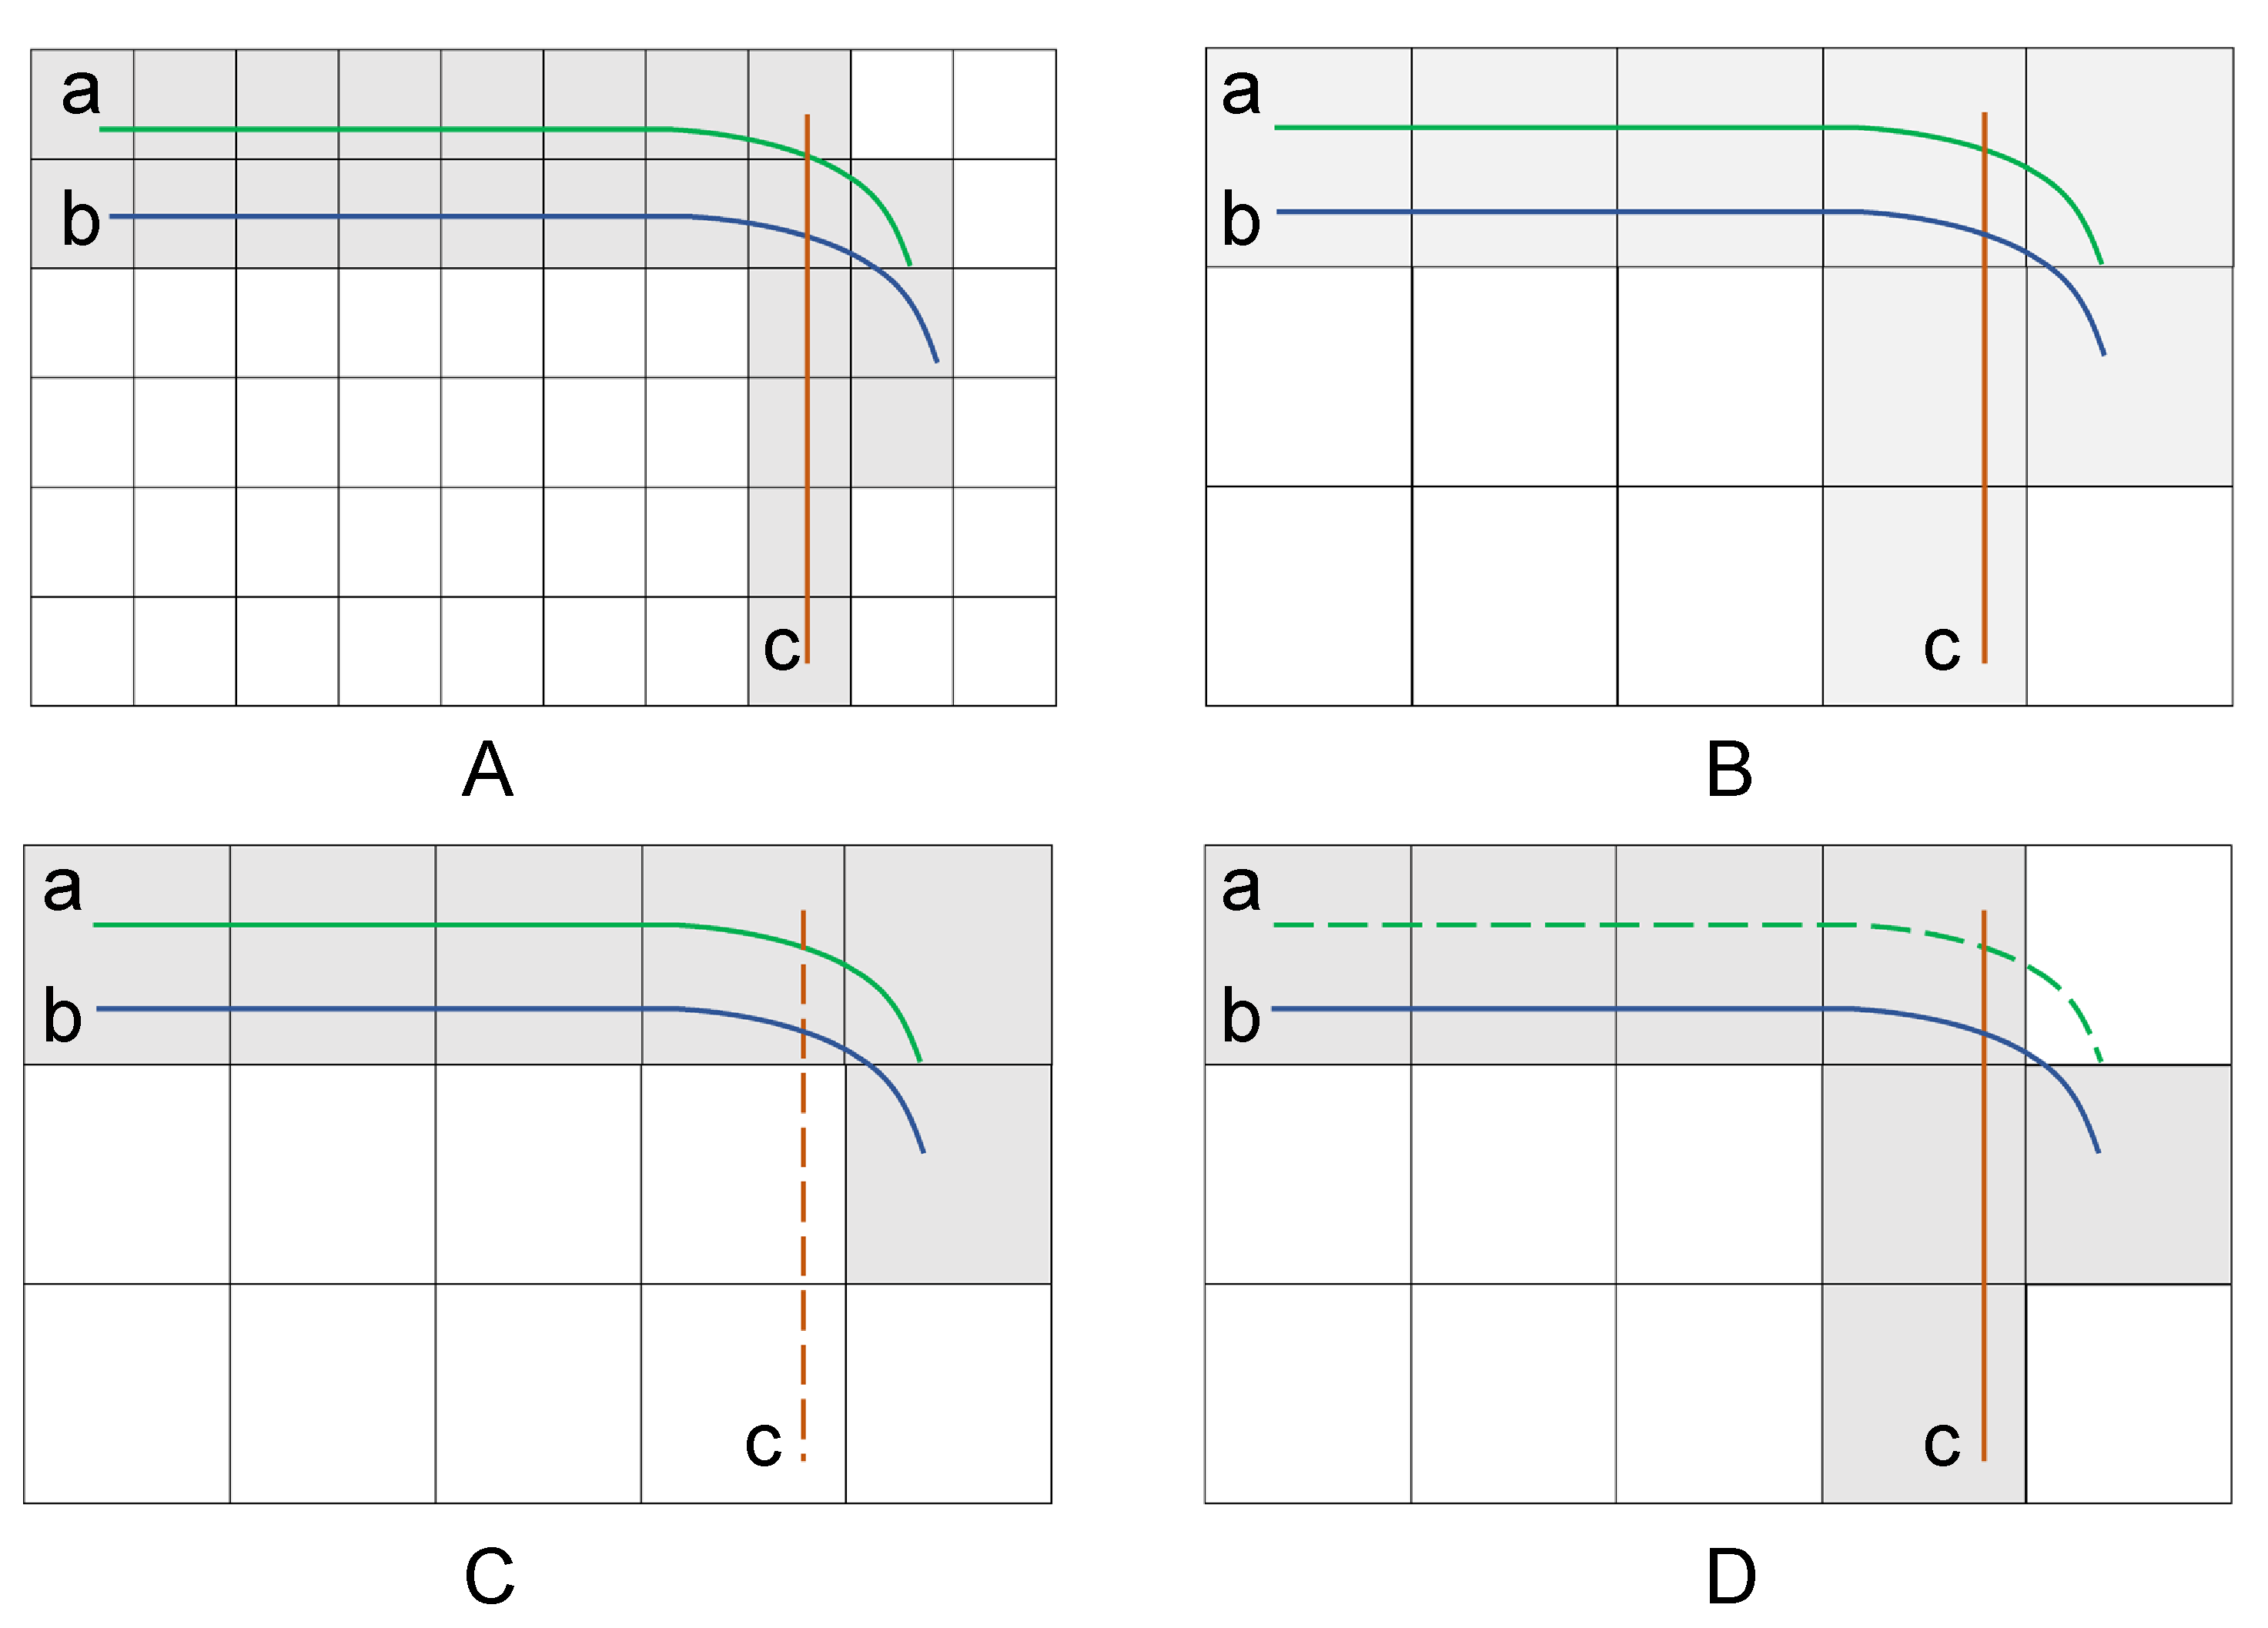
\includegraphics[width=0.4\textwidth]{pictures/problemsolveing/one_to_many.pdf}
%	\vspace{-5mm}
%	\caption{Resolution inconsistency}
%	\vspace{-5mm}
%	\label{fig:one_to_many}
%\end{figure}


% several notes for Bo, we should confirm them before submission:
% (1) rendering time,
% (2) gleaning insight from overview figures, i.e., low zoom level
% (3) delivers significantly richer information
% (4) arbitrary zooming resolutions





\section{Advance Approach: $\avats$}\label{sec:aa}
Until now, $\vats$ in Algorithm~\ref{alg:greedy} offers a visual fidelity guaranteed sampling approach for large-scale trajectory visualization problem (see Problem~\ref{prob:def}),
which returns the visual fidelity guaranteed result efficiently via the optimization techniques in Section~\ref{sec:opt}.
It means that the challenges (i) large trajectory dataset and (ii) limited rendering ability of graphics device (see Section~\ref{sec:intro}) have been addressed.
In this section, we focus on the third challenge of it, i.e.,  visual clutter.
In particular, we devise an advance approach $\avats$ to alleviate it by considering
(i) trajectory data distribution, and (ii) human perception ability.
We elaborate (i) and (ii) by the examples in Fig.~\ref{fig:delta} shortly.

\stitle{Trajectory data distribution} Considering \pt{} trajectory dataset, Fig.~\ref{fig:delta}(A) is the visualization result of $\vats$ with sampling ratio $0.5\%$.
Obviously, the real-world trajctory dataset is non-uniform distributed.
For example, the trajectories in the dense region is much more than these in the sparse region, as illustrated by the rectangles in Fig.~\ref{fig:delta}(A).

\stitle{Human perception ability} Intuitively, it is much easier for humans to distinguish the difference between sparse regions rather than dense regions in Fig.~\ref{fig:delta}(A) and (B).
The core reason is the perception capability of human beings is limited.
In particular, the visual difference of human beings will be diminished when the visualized trajectories is large enough with a given level of details,
i.e., the difference between two dense regions in Fig.~\ref{fig:delta}(A) and (B).

%instead of measuring the contribution of each trajectory w.r.t the selected trajectories in $\oR$ directly,
Taking the above two observations into consideration, the returning result of visual fidelity guaranteed sampling approach $\vats$ could be further improved by
delivering richer information at sparse regions and reducing visual clutter in dense regions.
In this section, we devise an advance approach $\avats$ (see Algorithm~\ref{alg:plus}) to achieve the above two objectives.
Specifically, we introduce perception tolerance parameter $\delta$ in $\avats$, which models human's perception capability at the most highest level of details.
In other words, suppose the pixel $(x,y)$ in canvas is covered by result set $\oR$ at the highest level,
the pixels around $(x,y)$, i.e., from $(x-\delta, y-\delta)$ to $(x+\delta, y+\delta)$, are not necessary to cover as they are in the perception tolerance of human beings.


Fortunately, we can slightly revise $\vats$ in Algorithm~\ref{alg:greedy} to incorporate the perception tolerance parameter $\delta$ in advance approach $\avats$, as shown in Algorithm~\ref{alg:plus}.
It measures the contribution of each trajectory $t_i$ w.r.t the selected trajectory set $\oR$'s augmented set $\oR^{+}$ (in Line~\ref{line:deltamax}).
The augmented set $\oR^{+}$ will be updated by the selected trajectory $tmp$ and its tolerance pixels set (in Line~\ref{line:delta}).

\vspace{-2mm}
\begin{algorithm}
    \caption{$\avats(\D,k=\alpha |\D|,\delta)$} \label{alg:plus}
    \begin{algorithmic}[1]
    \State Initialize result set $\oR \leftarrow \emptyset$
    \State Initialize augmented result set $\oR^{+} \leftarrow \emptyset$
    \While{$|\oR| < k$}
        \State $tmp \leftarrow argmax_{t_i \in \D} \oR^{+} \cup t_i$ \label{line:deltamax}
        \State $\oR \leftarrow \oR \cup \{ tmp \}$
        \State $\oR^{+} \leftarrow \oR^{+} \cup \mathsf{augment}(tmp, \delta)$\label{line:delta}
    \EndWhile
    \For{each $t$ in $\D$} \Comment{Representative encoding} \label{line:s}
        \State $tr \leftarrow argmin_{t_i \in \oR}{\mathsf{augment}(t_i, \delta) - t}$
        \State $tr.\mathsf{cnt}++$ \label{line:e}
    \EndFor
    \State Return $\oR$
    \end{algorithmic}
\end{algorithm}
\vspace{-2mm}

Interestingly, the visual clutter large trajectory visualization problem can be further reduced
by encoding representative trajectories in $\oR$ (the returning result of the advance approach $\avats$) with colors.
In particular, $\avats$ selects the trajectory which has largest uncovered pixels by taking human's perception tolerance capability into account at each iteration,
instead of only choosing the trajectory with largest uncovered pixels in $\vats$ (see Algorithm~\ref{alg:greedy}).
During its selection process, some of trajectories will not be included into the result set $\oR$ even they have more uncovered pixels w.r.t. $\oR$.
The reason is their uncovered pixels are too close to the pixels in the selected trajectories, i.e., within the tolerance area of selected pixels.
Taken Fig.~\ref{fig:zoom}(A) as example, suppose $\delta=1$ and trajectory $a$ was selected at the first iteration,
the selected trajectory in the second iteration is $c$ instead of $b$ as almost all pixels in $b$ is in the tolerance area of $a$'s.

Inherently, the $\avats$ trajectory selection process embeds the representativeness of each trajectory in the result set $\oR$.
We define the representativeness of a trajectory as the number of influenced trajectories in the dataset $\D$.
We compute the representativeness of each trajectory in $\oR$ from Line~\ref{line:s} to Line~\ref{line:e} in Algorithm~\ref{alg:plus}, then visualize them by encoding with different colors.
Fig.~\ref{fig:delta}(C) shows the visualized result of the  advance approach $\avats$ by encoding the trajectory representativeness with colors.
Obviously, the trajectories in dense region have deeper color than these in sparse regions as there many trajectories in dense region, thus the selected trajectories in the dense region are more representative.

\begin{figure}[t]
	\centering
	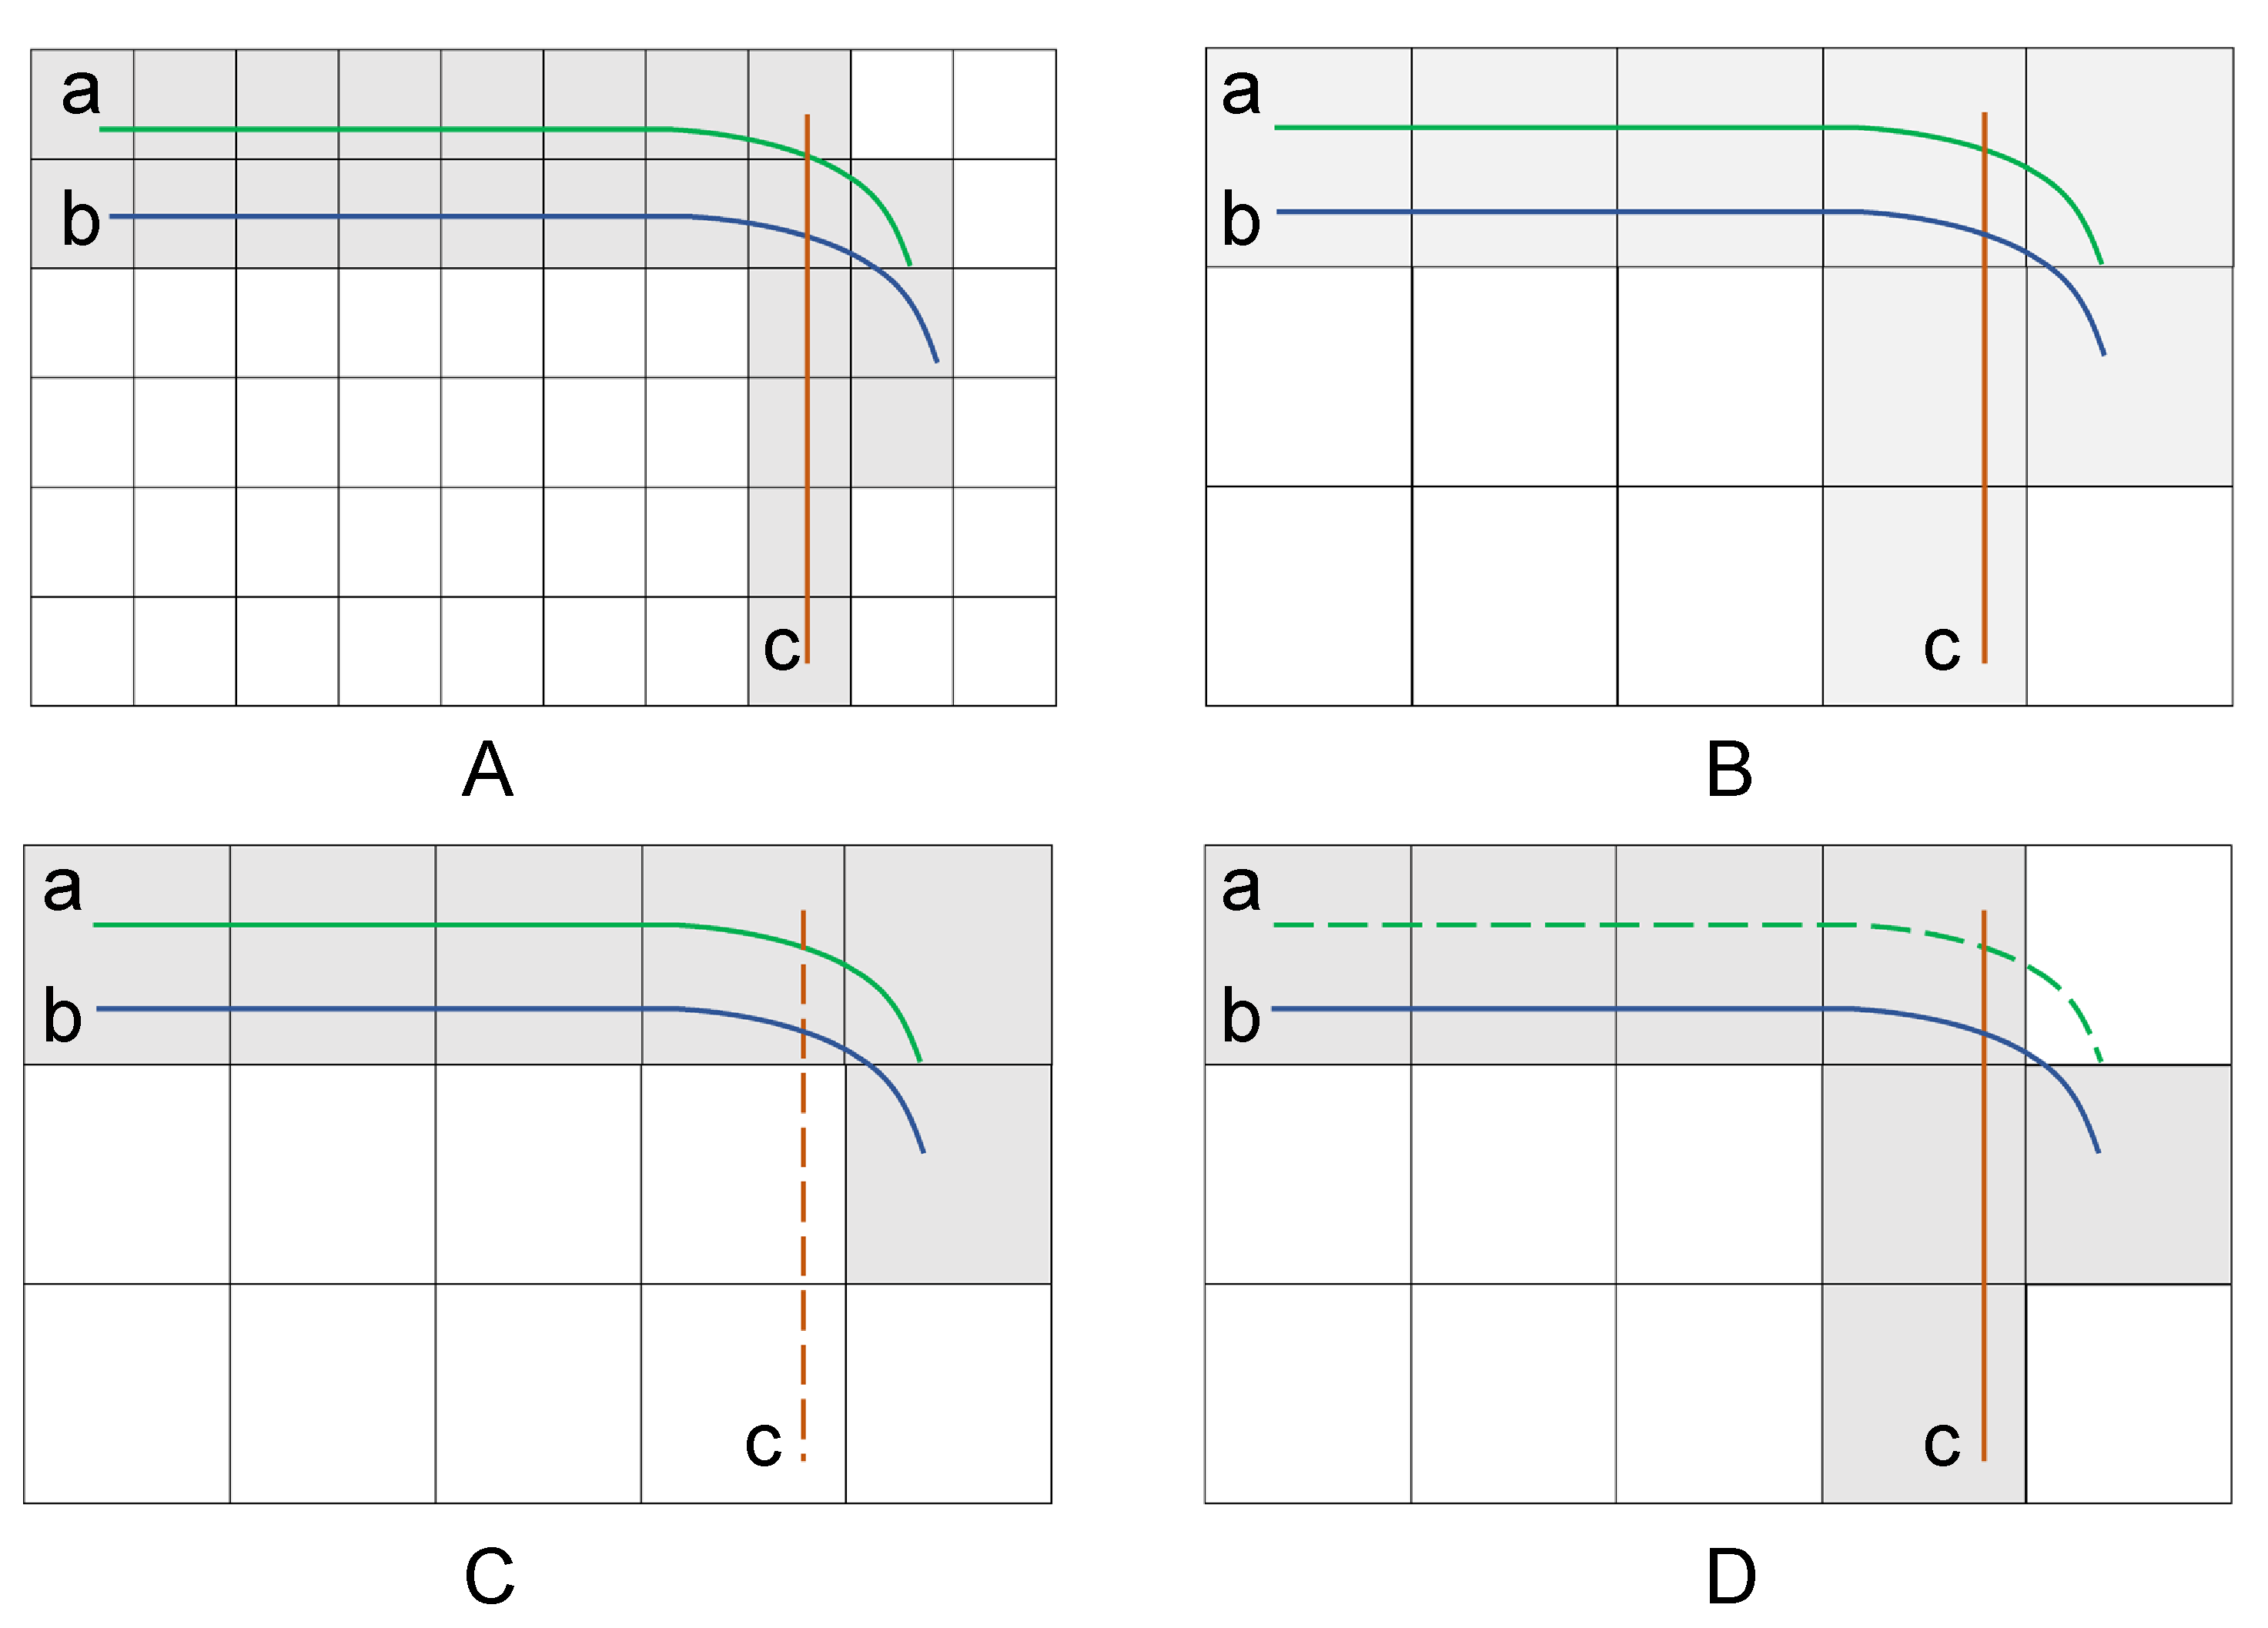
\includegraphics[width=0.4\textwidth]{pictures/problemsolveing/one_to_many.pdf}
	\vspace{-3mm}
	\caption{An illustration of $\avats$ with different zoom levels}
	\label{fig:zoom}
    \vspace{-6mm}
\end{figure}

Last but not least, it is worth to point out that our advance approach $\avats$ provides excellent visual fidelity over $\vats$ at arbitrary zooming resolutions naturally.
The key technique to achieve that is it considers the zooming resolutions inherently when introducing the perception tolerance $\delta$.
Take Fig.~\ref{fig:zoom} as an example, %Figure~\ref{fig:zoom}(A) and (B) show two different zoom-levels.
the zoom level in Fig.~\ref{fig:zoom}(A) is higher than it in Fig.~\ref{fig:zoom}(B).
As our above elaboration, our advance approach $\avats$ selects trajectory $a$ and $c$ at Fig.~\ref{fig:zoom}(A).
When it zoomed out, as shown in Fig.~\ref{fig:zoom}(b), it still captures the main sketch of the underlying dataset (as gray cells shown).




%(1) Richer Information Delivering: details aware; so Arbitrary zooming resolutions
%(2) Popularity Embedding: visual clutter



%\subsection{One-to-many strategy}~\label{sec:one_to_many}
%Since we detect the covered pixels in the highest level, two trajectories may be very close to each other but share very few pixels, which will lead to more information loss in the low zoom view as figure~\ref{fig:one_to_many}.
%We next elaborate a ``one-to-many'' strategy to further optimize the visual quality of our proposed technique.
%Recalling we use the highest zoom level to define the pixel size in the canvas.
%Thus, our visual quality guaranteed sampling algorithm is zoom-level oblivious, e.g., it guarantees the visual quality of result set $\oR$ at every zoom level.
%However, users always do not use/need the highest zoom level in visualization applications.
%For example, Google map shows city and streets at zoom level 1 and 15, respectively~\footnote{\url{https://developers.google.com/maps/documentation/}}.
%Motivated by the above observation, we devise ``one-to-many'' strategy by introducing a visual tolerance parameter $\delta$ to optimize the visual quality for users.
%Specifically, ,
%the ``one-to-many'' strategy will ignore all the pixels around $(x,y)$ within $\delta$ offset distance, i.e., all pixels from $(x-\delta, y-\delta)$ to $(x+\delta, y+\delta)$ will be skipped.
%We will demonstrate the effectiveness of the visual tolerance $\delta$ in experimental evaluations.
%
%%https://developers.google.com/maps/documentation/maps-static/dev-guide#Zoomlevels
%\begin{figure}[t]
%	\centering
%	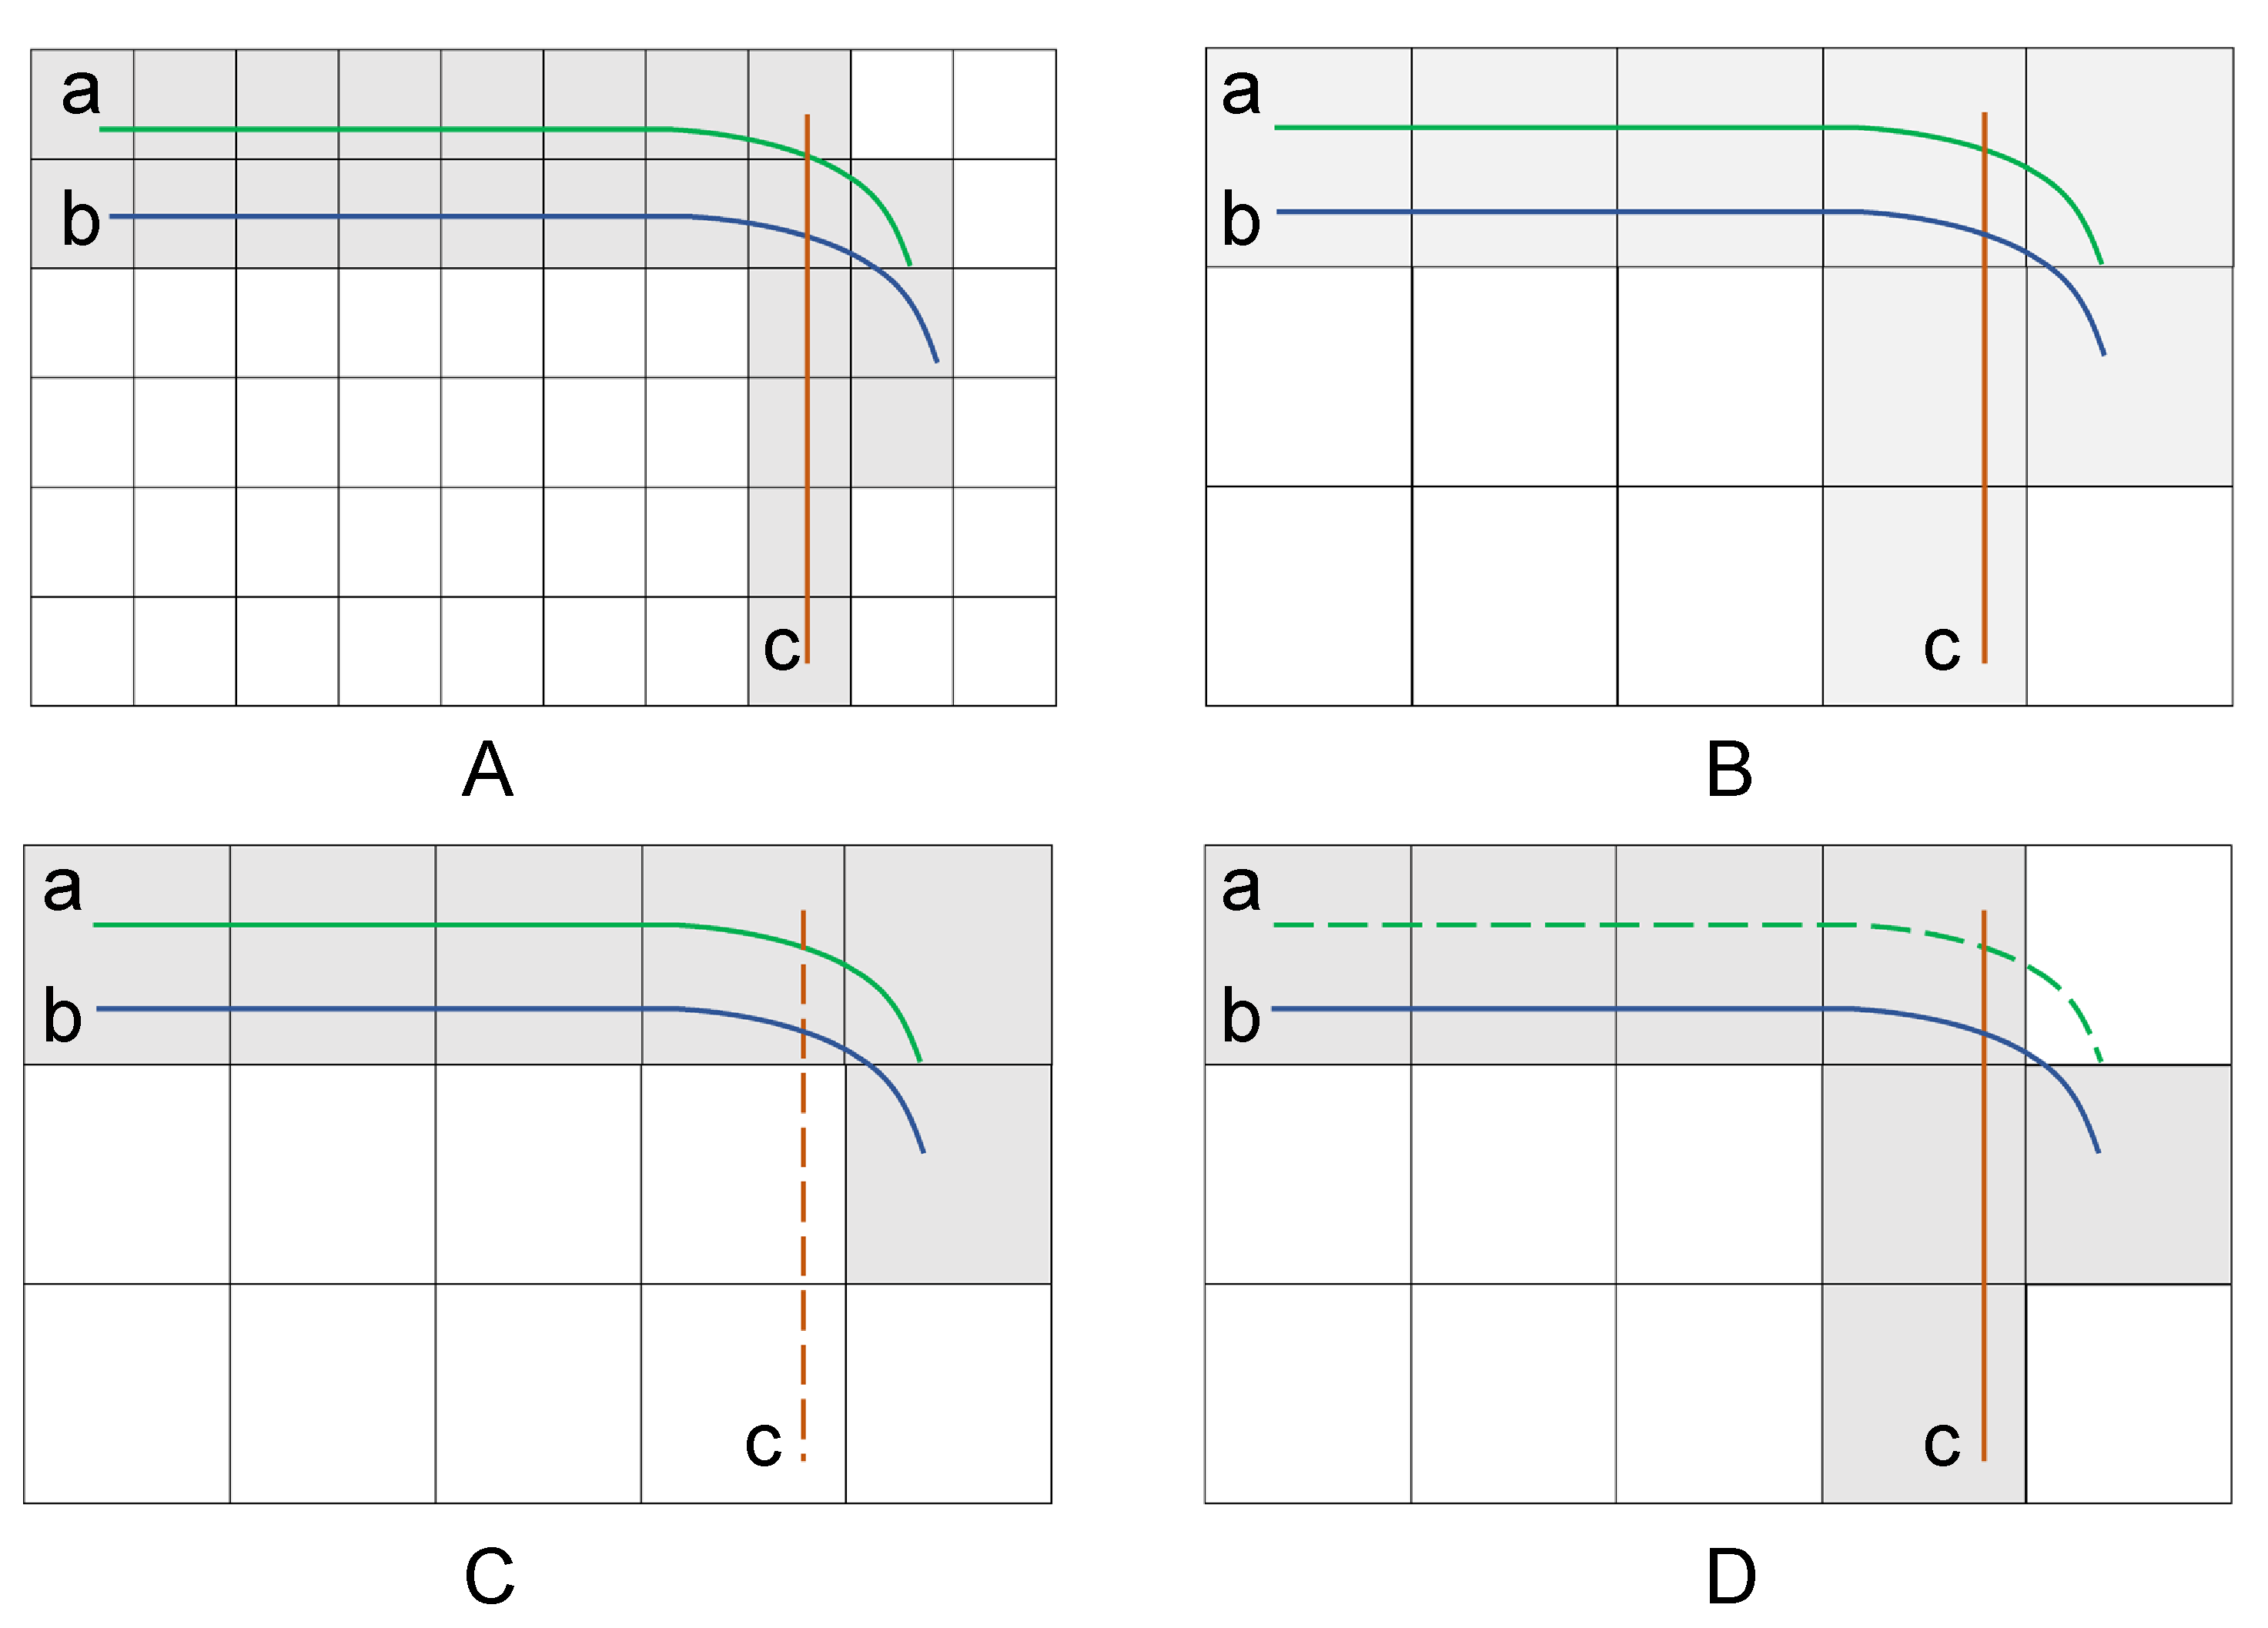
\includegraphics[width=0.4\textwidth]{pictures/problemsolveing/one_to_many.pdf}
%	\vspace{-5mm}
%	\caption{Resolution inconsistency}
%	\vspace{-5mm}
%	\label{fig:one_to_many}
%\end{figure}


%Specifically, $\avats$ incorporates a parameter $\delta$ during trajectory selection process in $\vats$ .
%In particular, we employ the parameter $\delta$ to model the end user's perception ability at the most high level of details.
%Surprisingly, our advance approach $\avats$ not only provides better visualization result when comparing with $\vats$ with the same sampling rate
%(e.g., Figure~\ref{fig:delta}(a) and (b) are the returning result of $\vats$ and $\avats$ respectively),
%but also embeds the popularity of selected trajectories by encoding the rest trajectories in the dataset in them,
%e.g., Figure~\ref{fig:delta}(c) is the visual result of $\avats$ with color encoded popularity.



%\vspace{-2mm}
\section{Evaluation}
We first applied our approaches to several real-world dataset and compare our method with the uniform random sampling. Then we conduct several user studies on specific analysis tasks. 
\subsection{Experimental results}
In this section, we will briefly evaluate our method by case studies. We will first make a brief comparison between the VQGTS and uniform random sampling at different granularities. Then we will show how VQGTS further improves the visual quality by taking the \QM{representative} into consideration. At last, we will extend our method to more dataset and demonstrate the effectiveness of propsoed method.
\subsubsection{VTGS and uniform random sampling}
Our first example uses taxi trajectories collected from 442 active taxis in the city of Porto, Portugal~\footnote{\url{http://www.geolink.pt/ecmlpkdd2015-challenge/dataset.html}}. Figure~\ref{fig:random_proposed} shows the comparison among the ground truth, uniform random sampling and the VQGTS. Both random sampling and VQGTS method take $0.01$ as the sampling rate. 
In the overview(map scale at 11), based on the ground truth(shown as figure~\ref{fig:random_proposed} A), the random sampling(shown as figure~\ref{fig:random_proposed} C) has a very poor the visual quality especially for the boundary region because very few trajectories are preserved by the sampling methods. That's because in the city, most of the taxi trips concentrate to the downtown, thus the sampled trajectories are more likely located in the downtown, which lead to a serious visual information loss.  
But our method(shown as figure~\ref{fig:random_proposed} B) are visually very close to the ground truth even in the margin regions. 
%In the overview, VQGTS(figure~\ref{fig:random_proposed} B) looks much more close to the ground truth(figure~\ref{fig:random_proposed} A) than the random method(figure~\ref{fig:random_proposed} C) especially for the boundary areas which . We further compare the details of region a and b. 
We further compare the visualization at the detail level(map scale at 15).
The figures in second rows depict the detail view of the ground truth, VQGTS and sampling at the region shown in Figure~\ref{fig:random_proposed} a, which is the city center of Porto. Comparing with VQGTS, random sampling preserve the general trajectory framework but miss the details(As the figure~\ref{fig:random_proposed}F, G shown). However, for the fridge of the city where the trajectories are spare distributed, the VQGTS has clear advantage than random sampling because it well preserve the detail structure of trajectories as shown in the black region in the figure~\ref{fig:random_proposed} H and I. This case demonstrates our proposed sampling method works well in both overview and detail view compared with the random sampling method.

\begin{figure}[t]
	\centering
	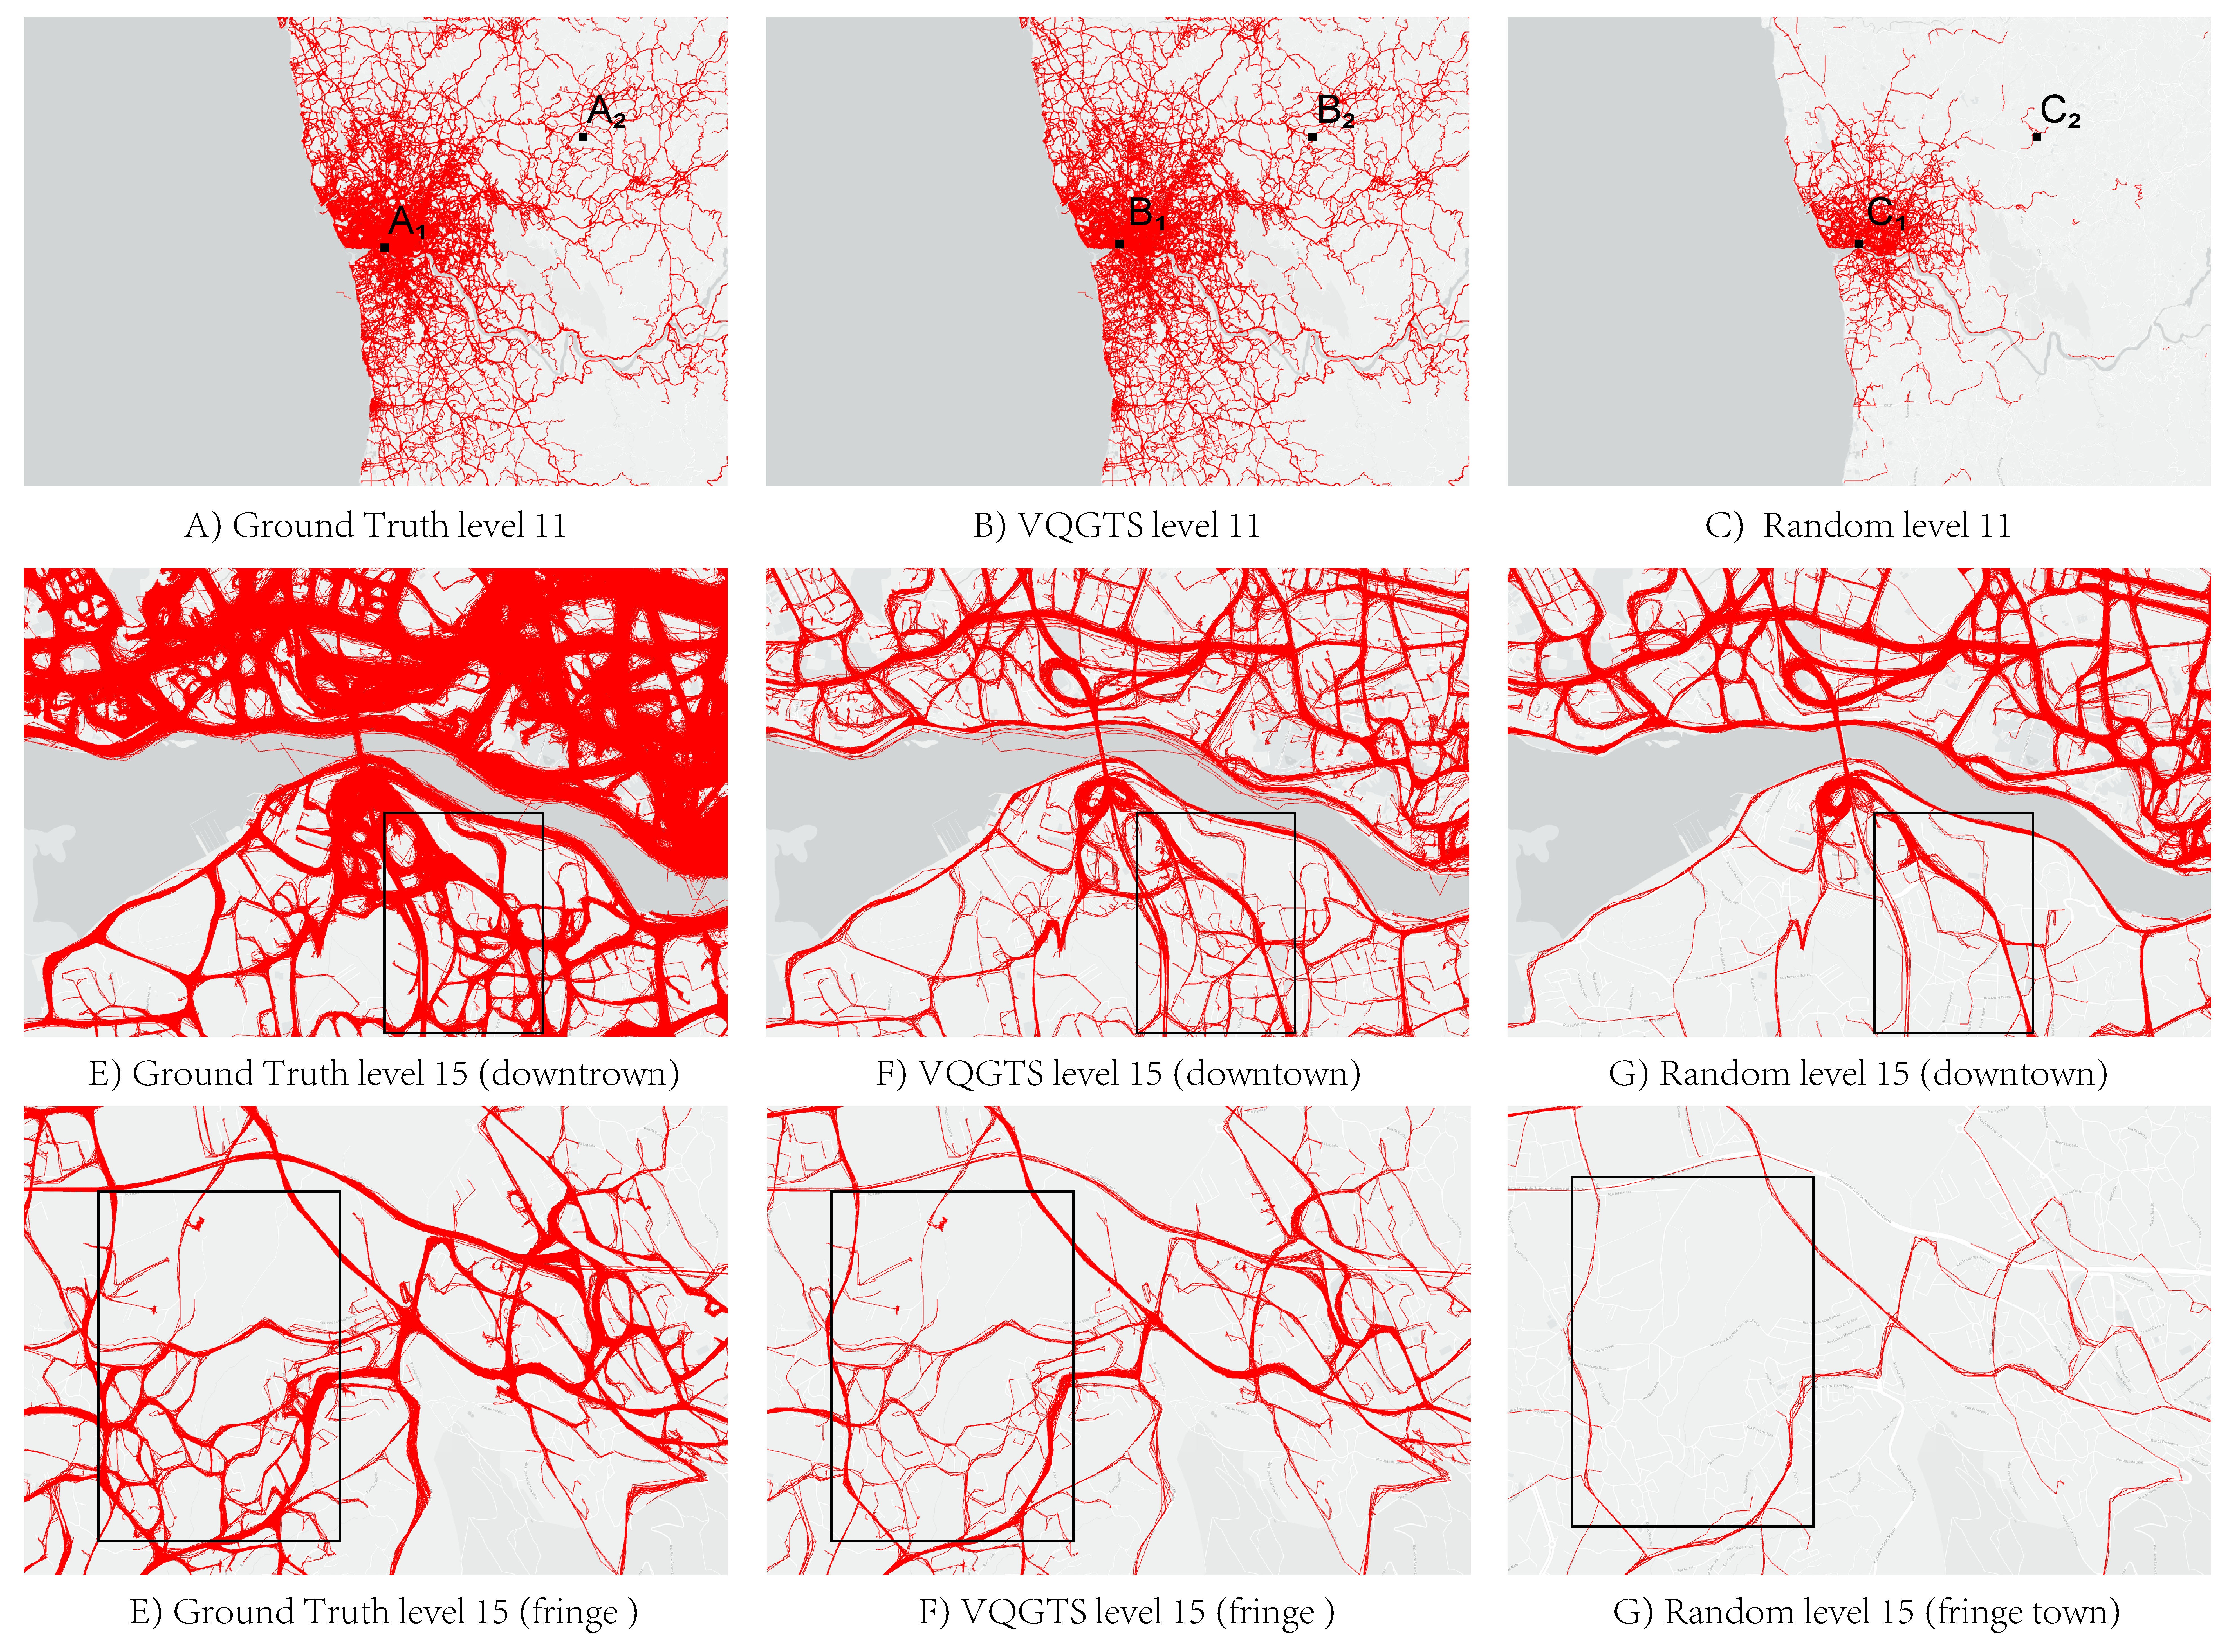
\includegraphics[width=0.48\textwidth]{pictures/experiment_study/Mehtod_resolution_study.pdf}
	\vspace{-5mm}
	\caption{Result evaluation between proposed method and uniform random sampling. The images in the three columns indicate the visualization results for full dataset, proposed method, and uniform random sampling respectively. The visualizations in the first row shows the overview. The visualizations in the second the third row indicate the detail level visualization of region 1 and region 2. }
	\vspace{-5mm}
	\label{fig:random_proposed}
\end{figure}

\subsubsection{Representativeness parameters analysis}
Figure~\ref{fig:heap} demonstrates the effectiveness of our method in the level of overview. The $\avats$ can preserve more details of the trajectory especially in the sparse regions and the $\avats$. We further explore how the value of $\delta$ affects the visualization results under different parameters including the spatial locations, the sampling rates and map resolution. Figure~\ref{fig:quality_chart} shows the overview of the visualization visual quality among all these parameters. The x axis indicate the map resolution from the detail view to overview(11~20). The y axis indicate the visual quality and the line with glyph indicate the sampling algorithms including uniform random sampling, $\vats$ and $\avats$ with different representative parameters. The figure shows the both $\vats$ and $\avats$ have better performance than random sampling and all of these linechart show the trend that from the detail view to the global view, the visual qualities keep increasing. 


\begin{figure}[t]
	\centering
	\vspace{2mm}
	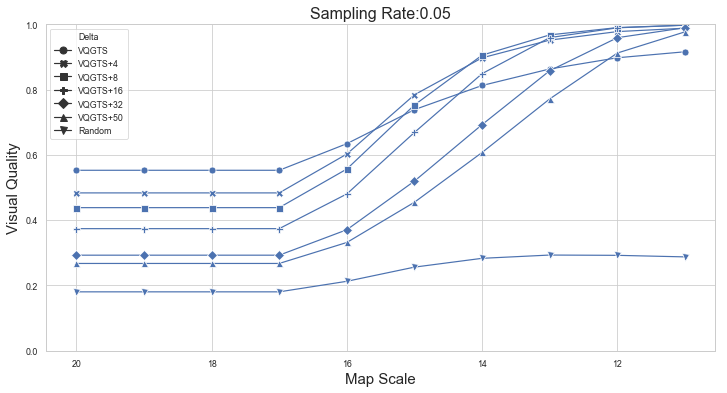
\includegraphics[width=0.48\textwidth]{pictures/experiment_study/quanlity.png}
	\caption{Visual quality chart. X axis indicates map scale from detail view to overview; y axis indicate the visual quality. }
	\vspace{0mm}
	\label{fig:quality_chart}
\end{figure}

\subsection{User study}
\setlist{nolistsep}
\begin{itemize}[noitemsep]
    \item Visual similarity
    \item Identify outliers
\end{itemize}

\subsection{Expert overview}


\vspace{-2mm}
\section{Conclusion and future work}~\label{sec:con}

Visualizing large trajectory dataset is challenge due to two reasons: visual clutter and long rendering time.
% The existing researches mostly focus on visual clutter issues by developing advanced data aggregation and interaction techniques.
Data sampling technique, an effective method in reducing the rendering time by shrinking the data size, has been applied in a variety of data.
However, very few work target at the trajectory sampling especially from the perspective of visualization.
The most commonly used sampling method, uniform random sampling technique, always generate results with very poor visual quality because very few trajectories located at margin regions can be preserved.
We fill the gap by proposing a novel sampling techniques $\avats$ which guarantees the visual quality at overview and reduce the visual clutter at the detail view. The technique characteristics and a series of parameters setting are discussed.
We compare $\avats$ with uniform random sampling in regarding to visual quality preservation and time-usage. We evaluate the effectiveness of proposed method by applying our method to different dataset and conducting users studies on specific interactive trajectory exploration tasks.


Even though it is recommended to use our method with caching techniques, our experience in the experiment shows that a faster algorithm will be more user friendly for the real world ad-hoc exploration tasks. For future work, we first plan to reduce the time usage by leveraging the advanced database techniques such as the indexing technique or use GPU acceleration. 
In addition, there are several directions can be further explored to enrich the information presented by the visualization. 
First we will develop different color encoding schema to present the spatial distribution of trajectory more precisely. 
In current schema, the color of one trajectory is the same, thus the color of the long trajectories may mislead the users because they pass  through many regions with different level of the traffic crowdedness. One solution is to use gradient color schema to encode the trajectories.
Another interesting direction is to extend the approach to support the mulit-class characteristics which is a commonly existed in variety of trajectory dataset.


\balance
%\bibliographystyle{abbrv}
\bibliographystyle{abbrv-doi}
%\bibliographystyle{abbrv-doi-narrow}
%\bibliographystyle{abbrv-doi-hyperref}
%\bibliographystyle{abbrv-doi-hyperref-narrow}

\bibliography{ref}
\end{document}

